\section{Apresentação do sistema}\label{sec:apresentacaoSistema}

Nesta seção, é apresentado o cliente \textit{web} desenvolvido para o gerenciamento de gado leiteiro, detalhando as interfaces e os comportamentos dinâmicos que compõem o fluxo de trabalho dos técnicos do \gls{IDR-PR}. O sistema foi projetado para oferecer uma experiência intuitiva, priorizando a clareza na visualização dos dados e a agilidade no registro de informações em campo.

\subsection{Autenticação e Registro de Técnicos}\label{subsec:apresentacaoLogin}

O acesso ao sistema inicia-se pela tela de autenticação (\autoref{fig:sys-login}), onde o técnico informa suas credenciais. Esta interface segue a identidade visual do \gls{IDR-PR}, garantindo que cada profissional acesse exclusivamente as propriedades sob sua responsabilidade técnica.

\begin{figure}[htpb]
  \centering
  \caption{Interface de Login}
  \label{fig:sys-login}
  
\includegraphics[width=0.8\textwidth]{figuras/sys-login.png}
  \fonte{Autoria própria (2026)}
\end{figure}

Para garantir a integridade dos dados desde o primeiro contato, todos os formulários do sistema utilizam validações rigorosas via biblioteca Zod. Na \autoref{fig:sys-cadastro-tecnico-validacao}, observa-se o comportamento do formulário de cadastro de técnicos ao detectar campos obrigatórios ausentes ou formatos inválidos após a tentativa de avanço para a próxima etapa. O sistema impede o envio à \gls{API} enquanto as pendências não forem resolvidas, fornecendo \textit{feedback} visual imediato.

\begin{figure}[htpb]
  \centering
  \caption{Validação de Campos no Cadastro de Técnicos}
  \label{fig:sys-cadastro-tecnico-validacao}
  
\includegraphics[width=0.8\textwidth]{figuras/sys-cadastro-tecnico-validacao.png}
  \fonte{Autoria própria (2026)}
\end{figure}

\clearpage

\subsection{Gestão de Propriedades e Navegação Modular}\label{subsec:apresentacaoPropriedades}

A listagem de propriedades (\autoref{fig:sys-propriedades}) é o ponto de partida para o trabalho técnico. Esta interface conta com um sistema de pesquisa global que utiliza a técnica de \textit{Debounce}, processando os filtros apenas após a interrupção da digitação para otimizar o uso da rede. A tabela permite a ordenação dinâmica por qualquer coluna (Produtor, Propriedade ou Município) e uma paginação fluida para navegação em grandes inventários.

\begin{figure}[htpb]
  \centering
  \caption{Listagem de Propriedades com Filtro e Ordenação}
  \label{fig:sys-propriedades}
  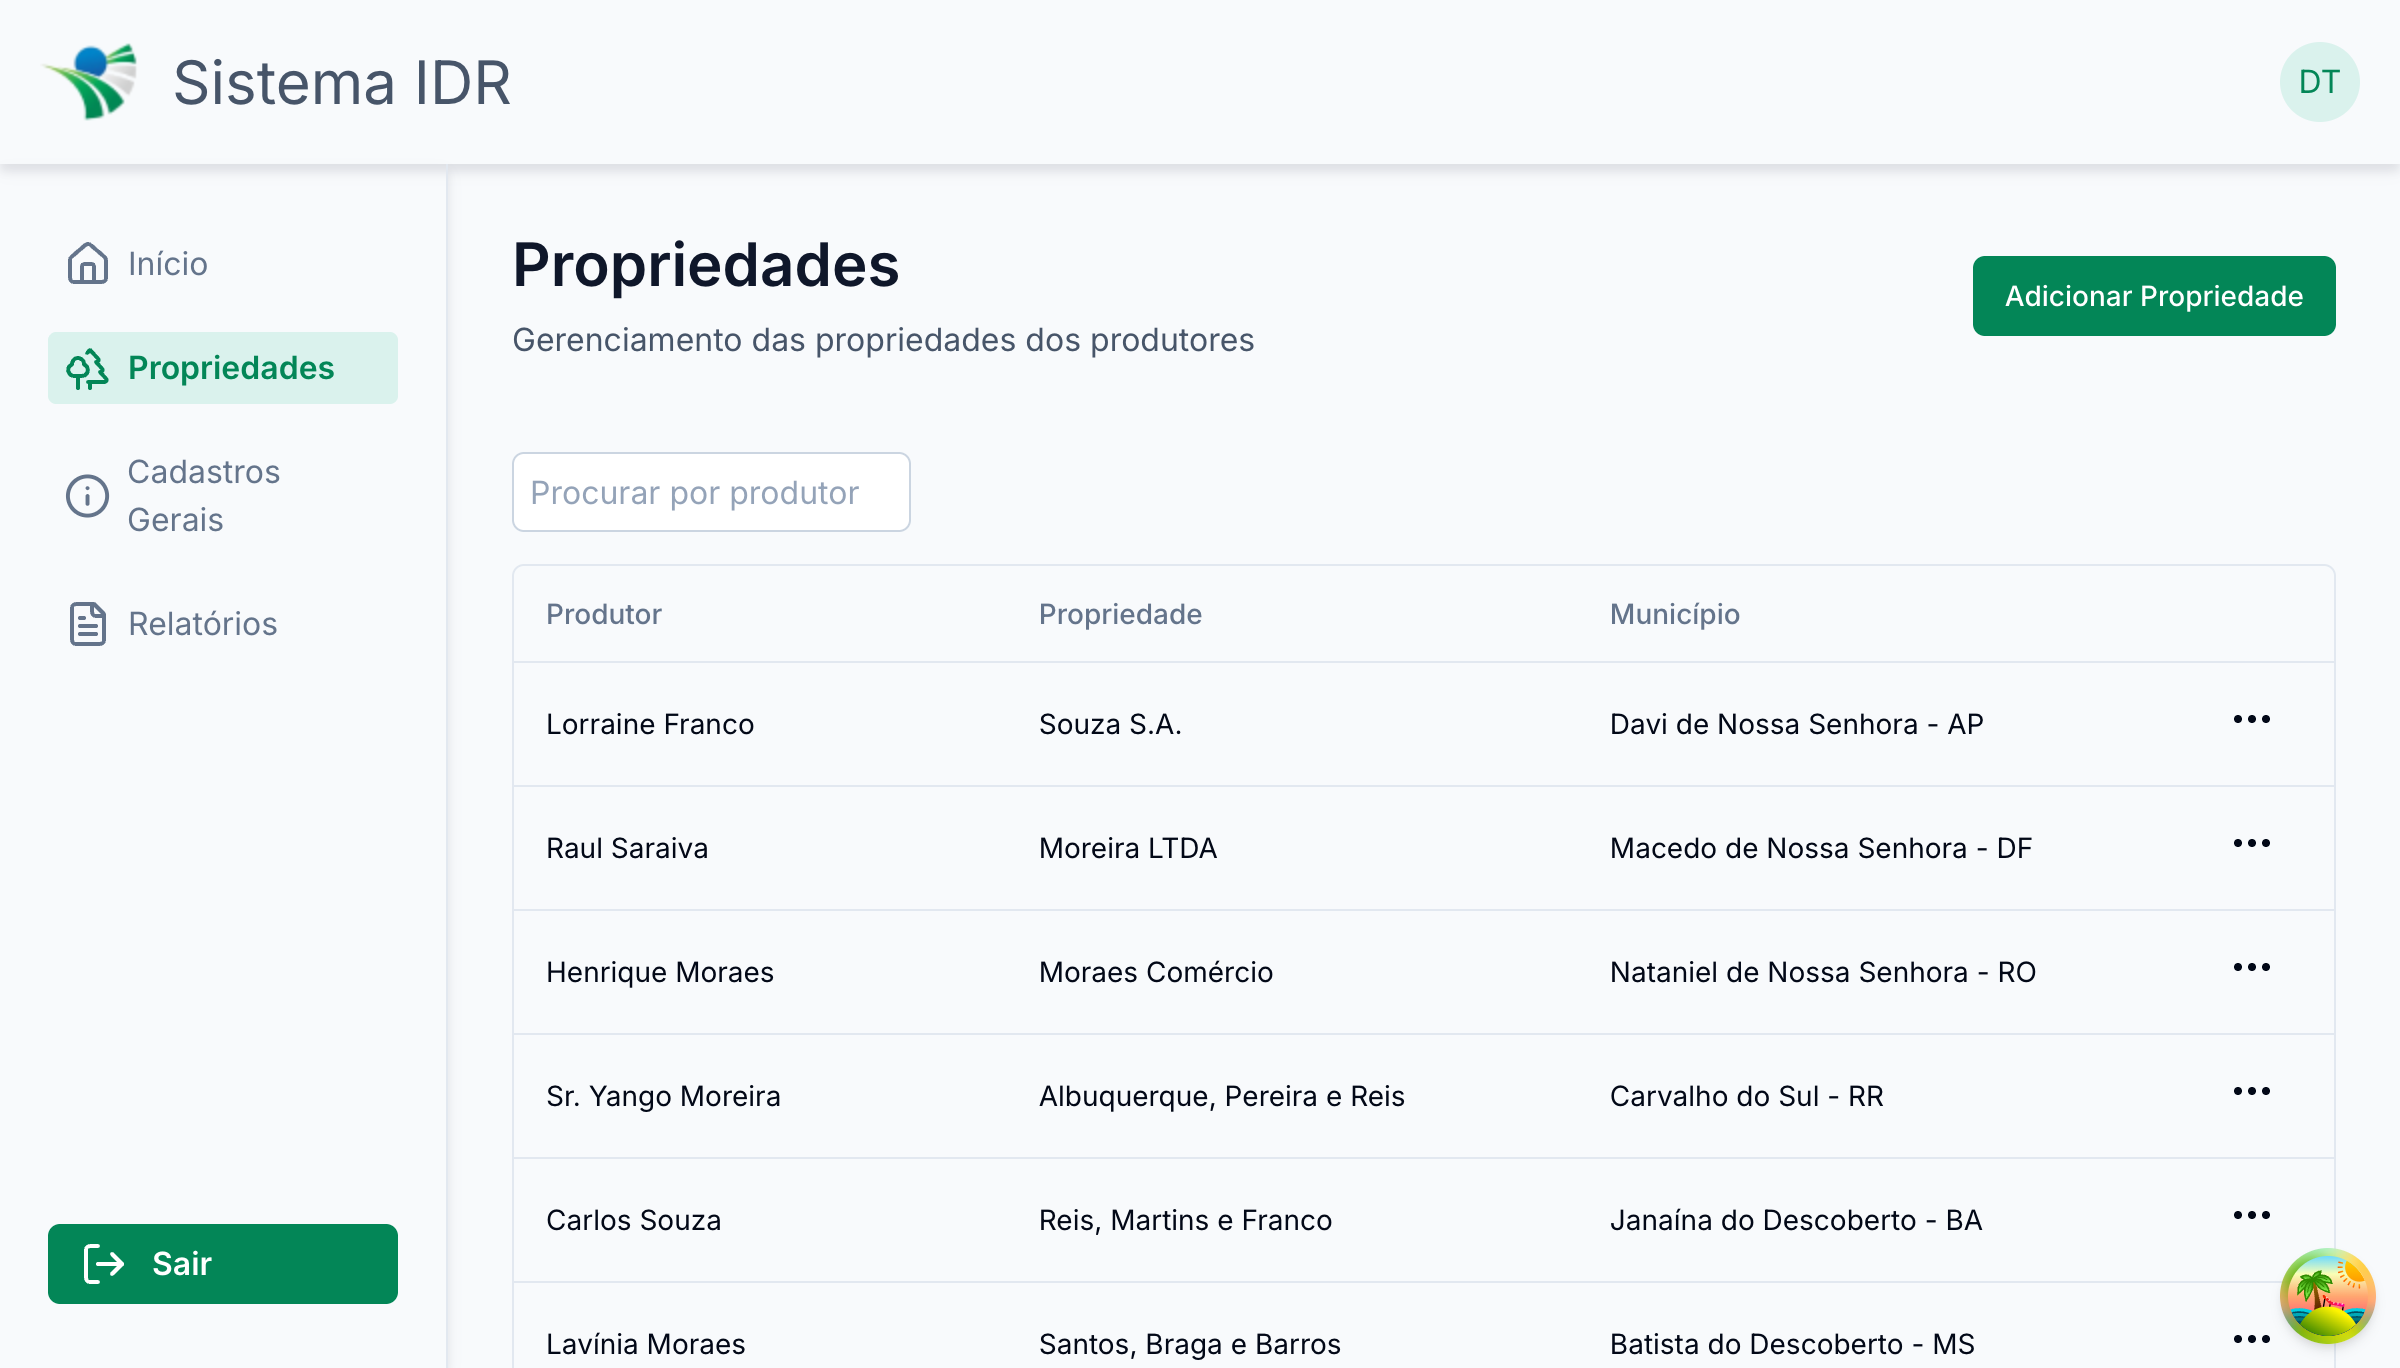
\includegraphics[width=0.8\textwidth]{figuras/sys-propriedades.png}
  \fonte{Autoria própria (2026)}
\end{figure}

Para navegar nos detalhes da propriedade, o técnico pode clicar na linha da propriedade que deseja acessar. Ao clicar, o sistema carrega o painel central (\autoref{fig:sys-propriedade-detalhes}), onde o cabeçalho exibe dinamicamente o nome da fazenda e do produtor. A interface é organizada em abas (Dados da Terra, Animais, Cultivos, etc.), permitindo que o técnico gerencie submódulos como máquinas e forrageiras sem perder o contexto da unidade produtiva.

\begin{figure}[htpb]
  \centering
  \caption{Painel da Propriedade com Cabeçalho Contextual e Abas}
  \label{fig:sys-propriedade-detalhes}
  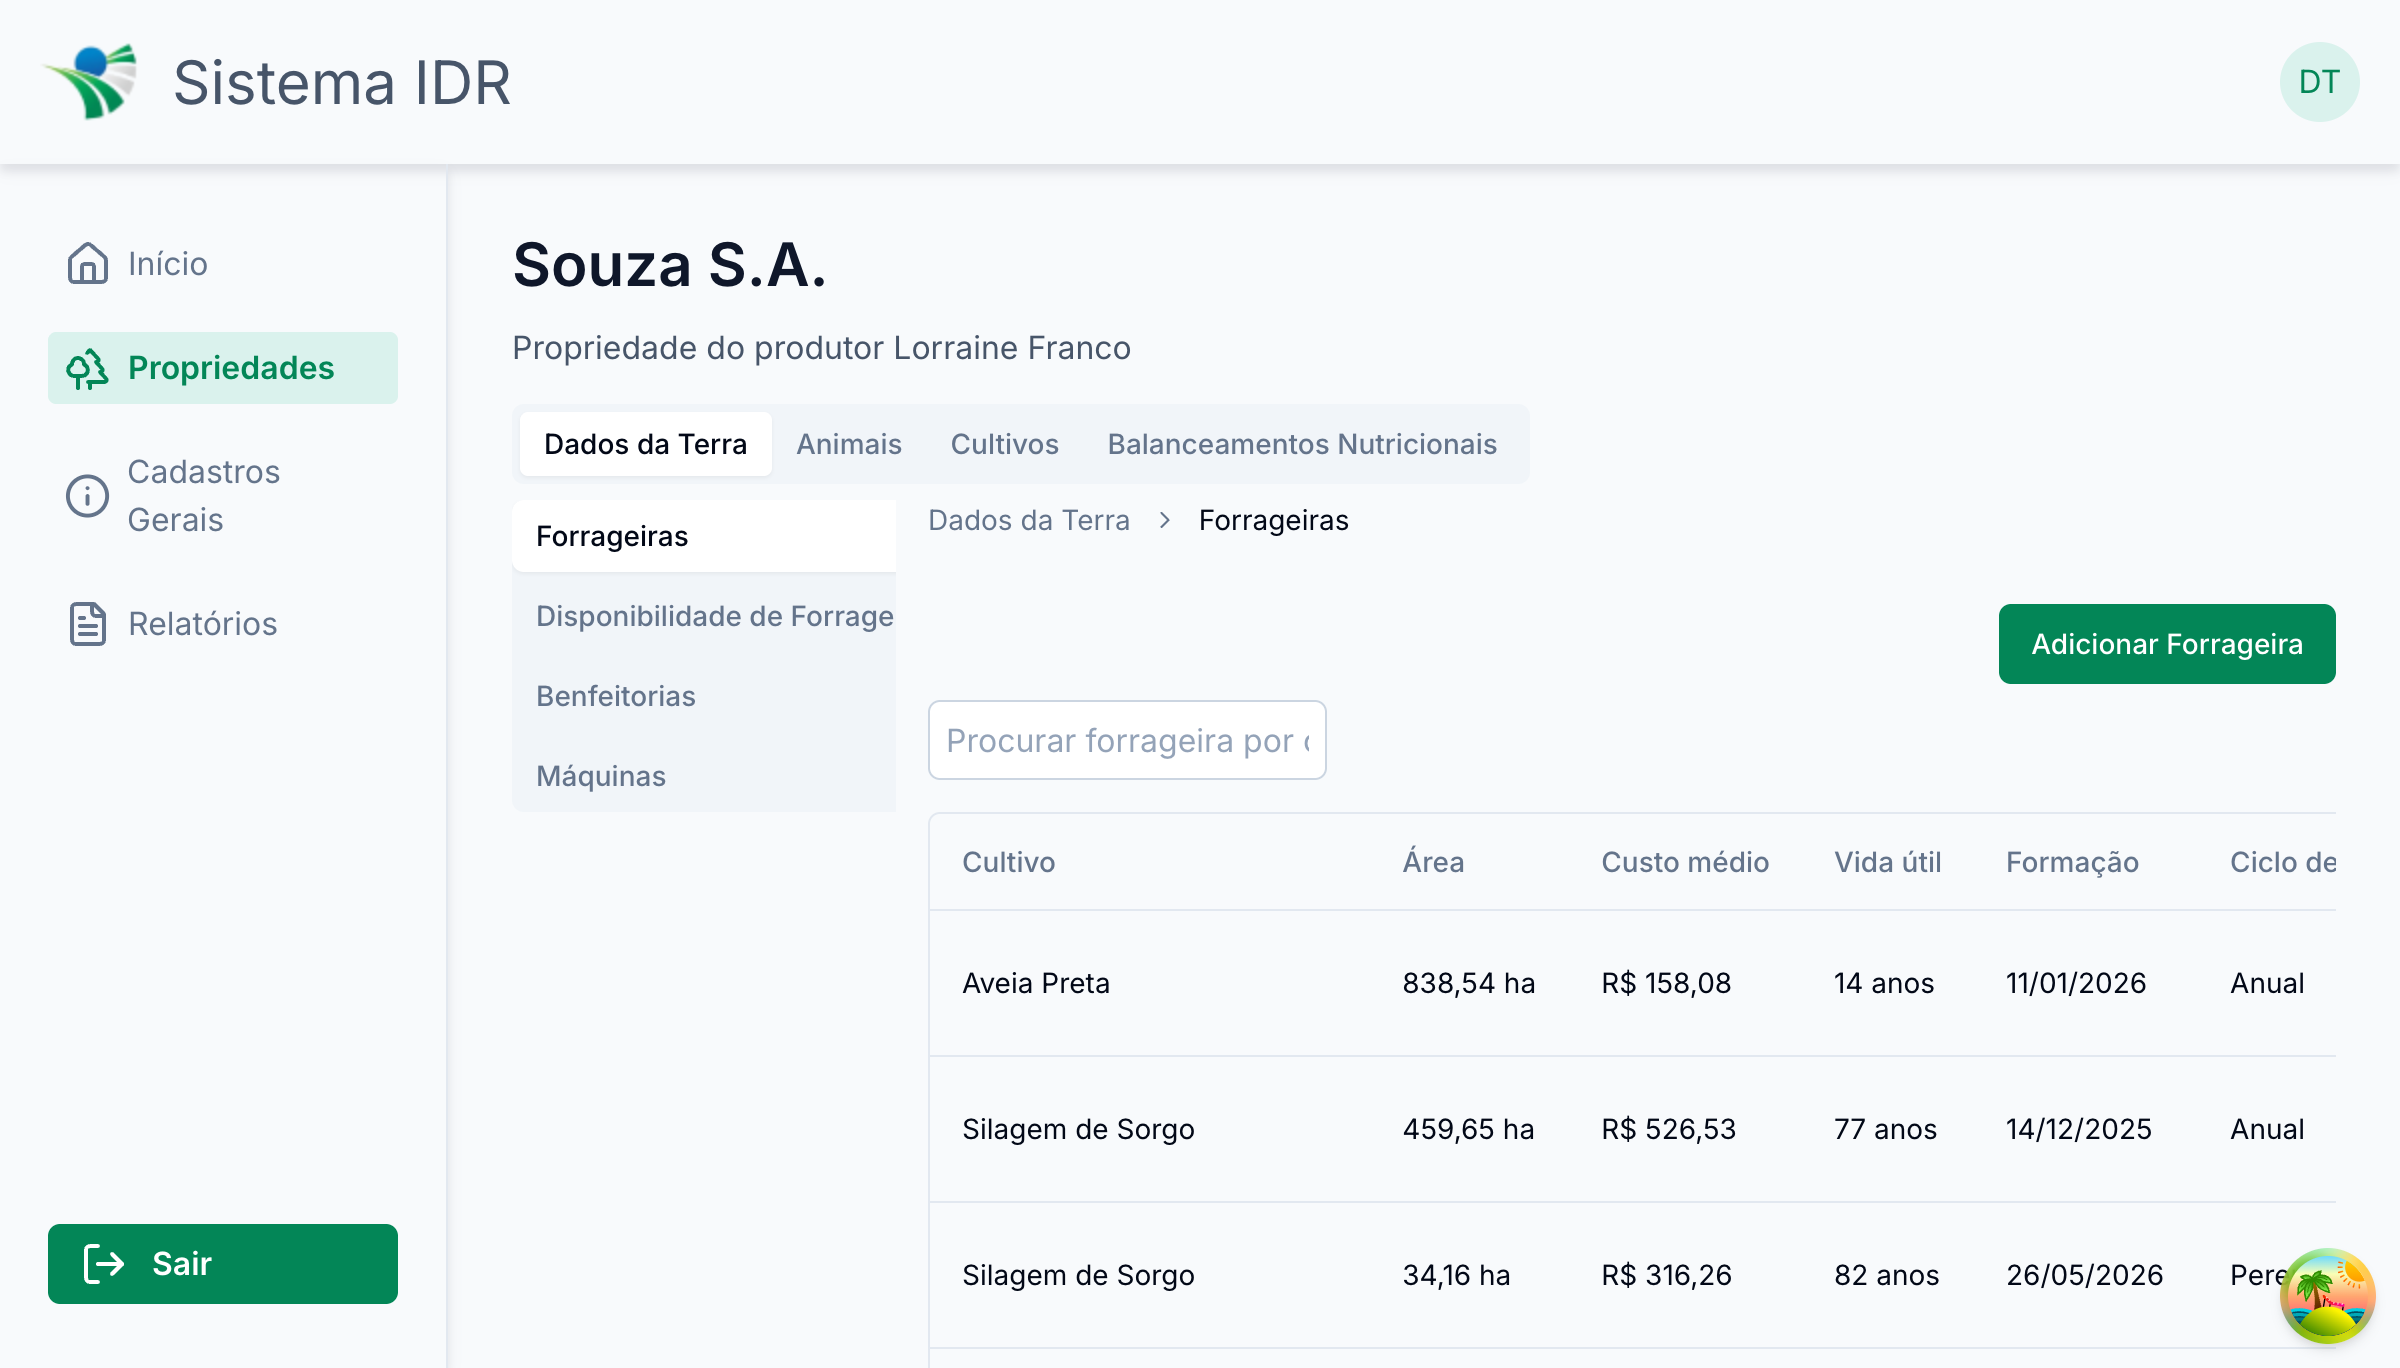
\includegraphics[width=0.8\textwidth]{figuras/sys-propriedade-detalhes.png}
  \fonte{Autoria própria (2026)}
\end{figure}

\clearpage

Para a expansão da base de dados, o sistema oferece um formulário de cadastro de propriedades estruturado em abas (\autoref{fig:sys-propriedade-cadastro}), onde informações de colaboradores e localização geográfica são coletadas de forma segregada, garantindo uma interface limpa e organizada.

\begin{figure}[htpb]
  \centering
  \caption{Cadastro de Nova Propriedade}
  \label{fig:sys-propriedade-cadastro}
  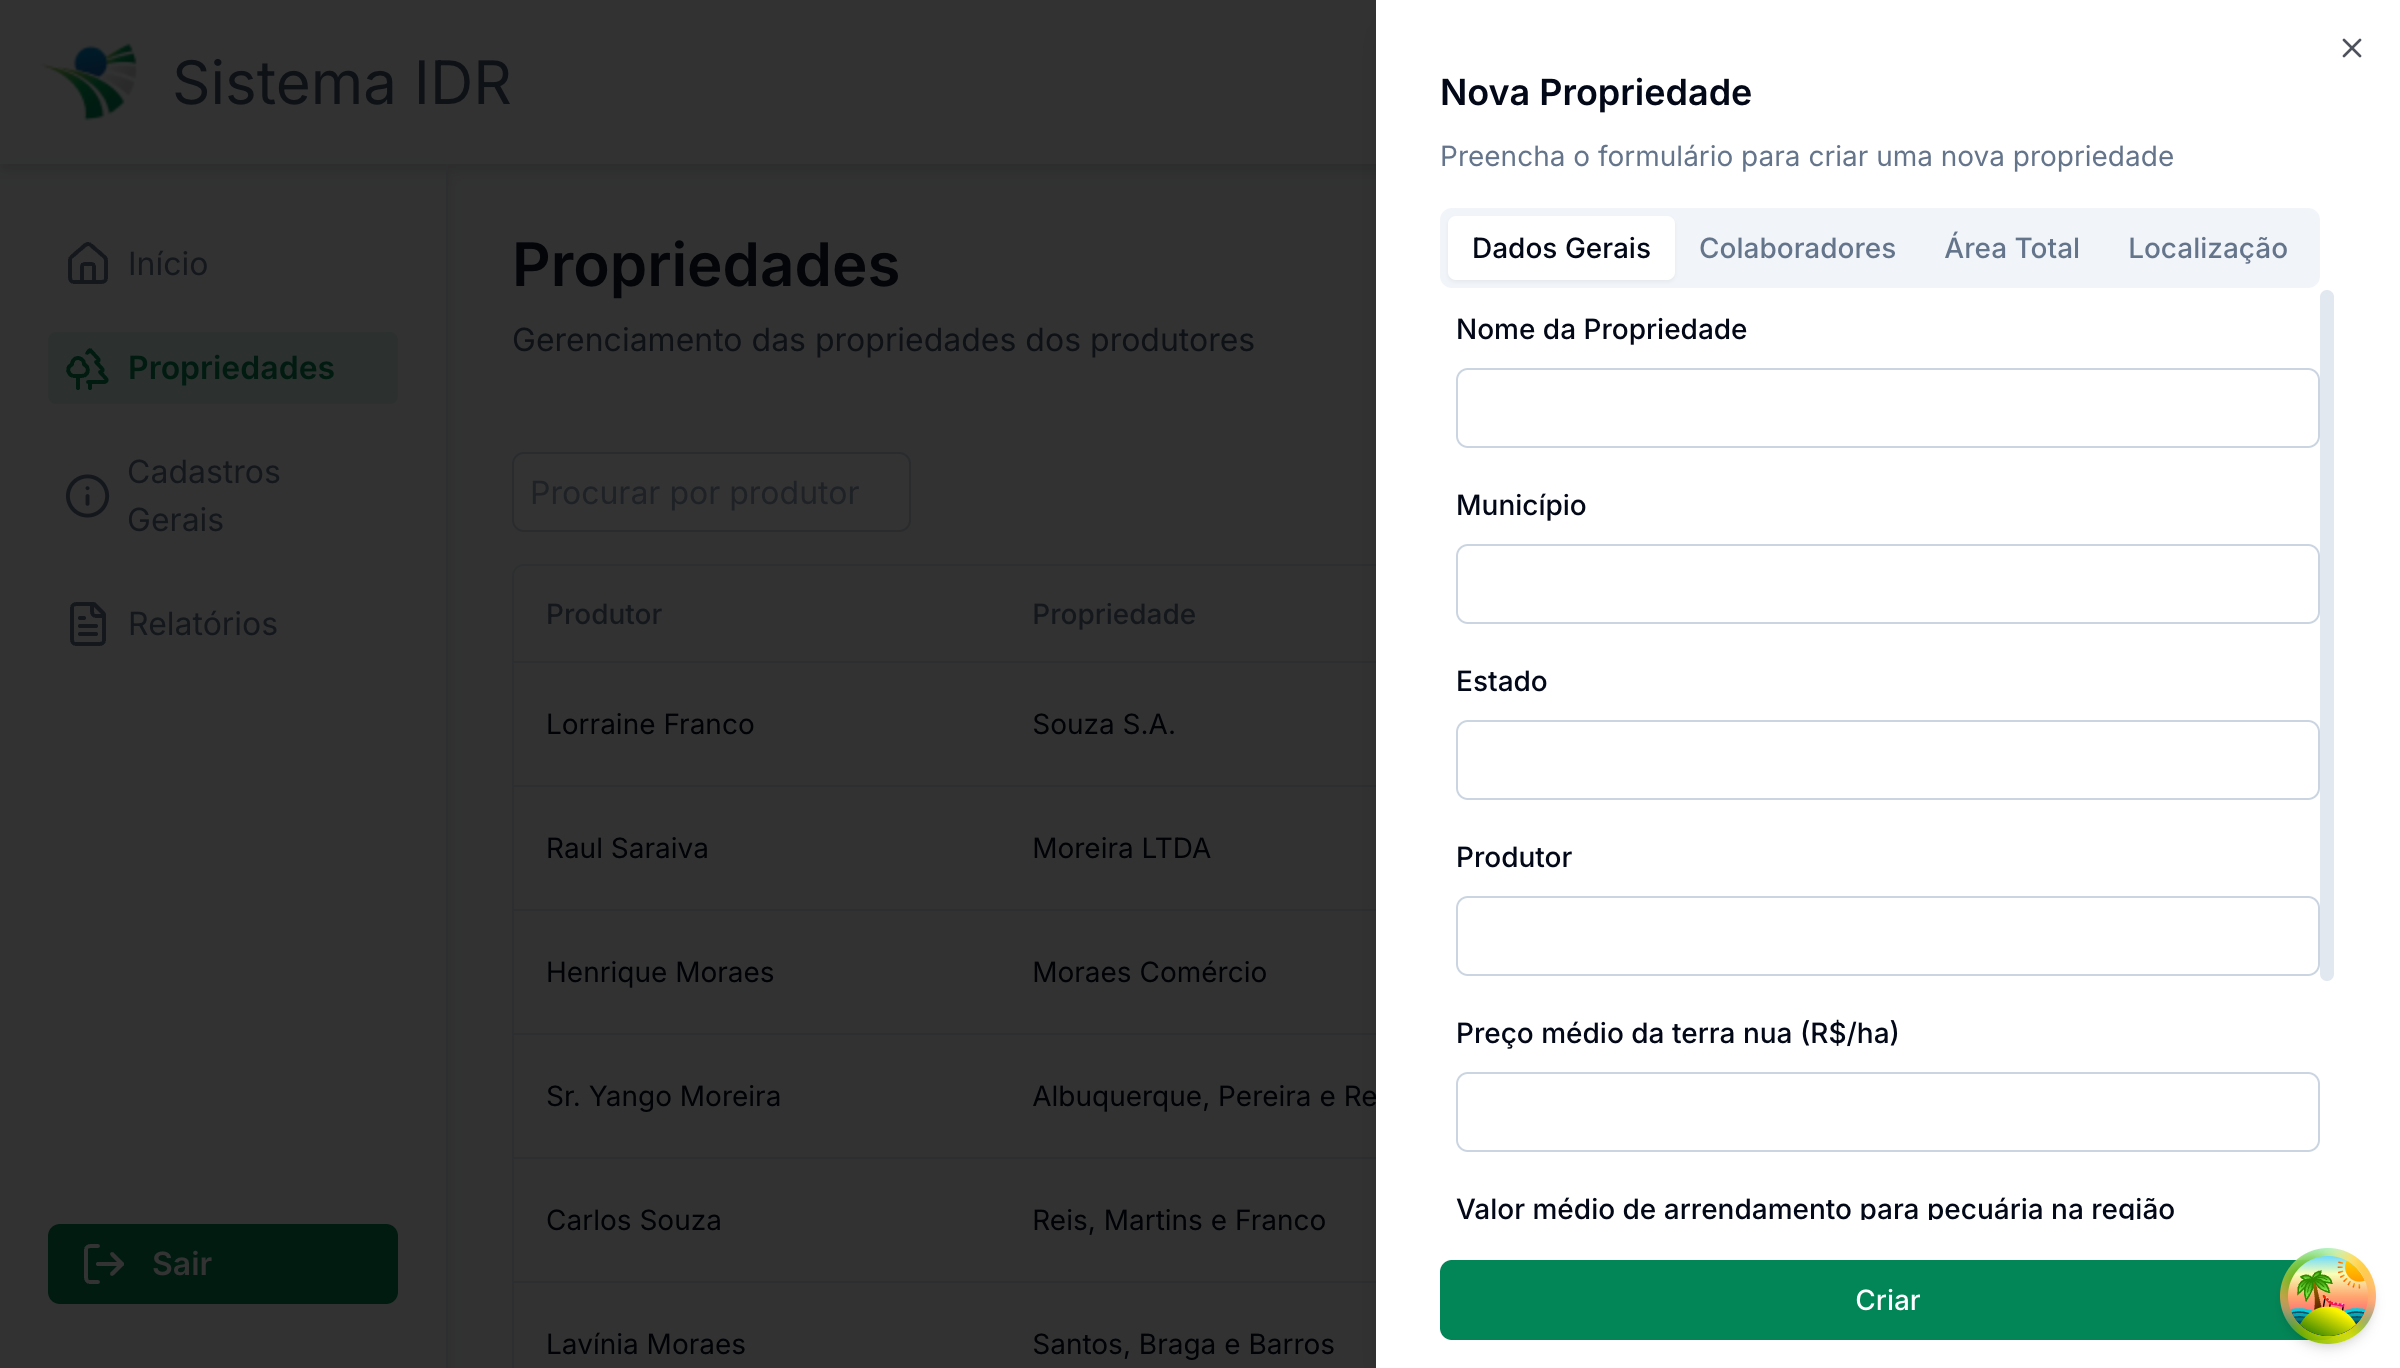
\includegraphics[width=0.8\textwidth]{figuras/sys-propriedade-cadastro.png}
  \fonte{Autoria própria (2026)}
\end{figure}

\clearpage

\subsection{Módulo de Animais}\label{subsec:apresentacaoAnimais}

A gestão do rebanho permite um controle cirúrgico do plantel por meio de uma interface dedicada (\autoref{fig:sys-animais}).

\begin{figure}[htpb]
  \centering
  \caption{Interface de Gestão de Animais com Identificação e Raça}
  \label{fig:sys-animais}
  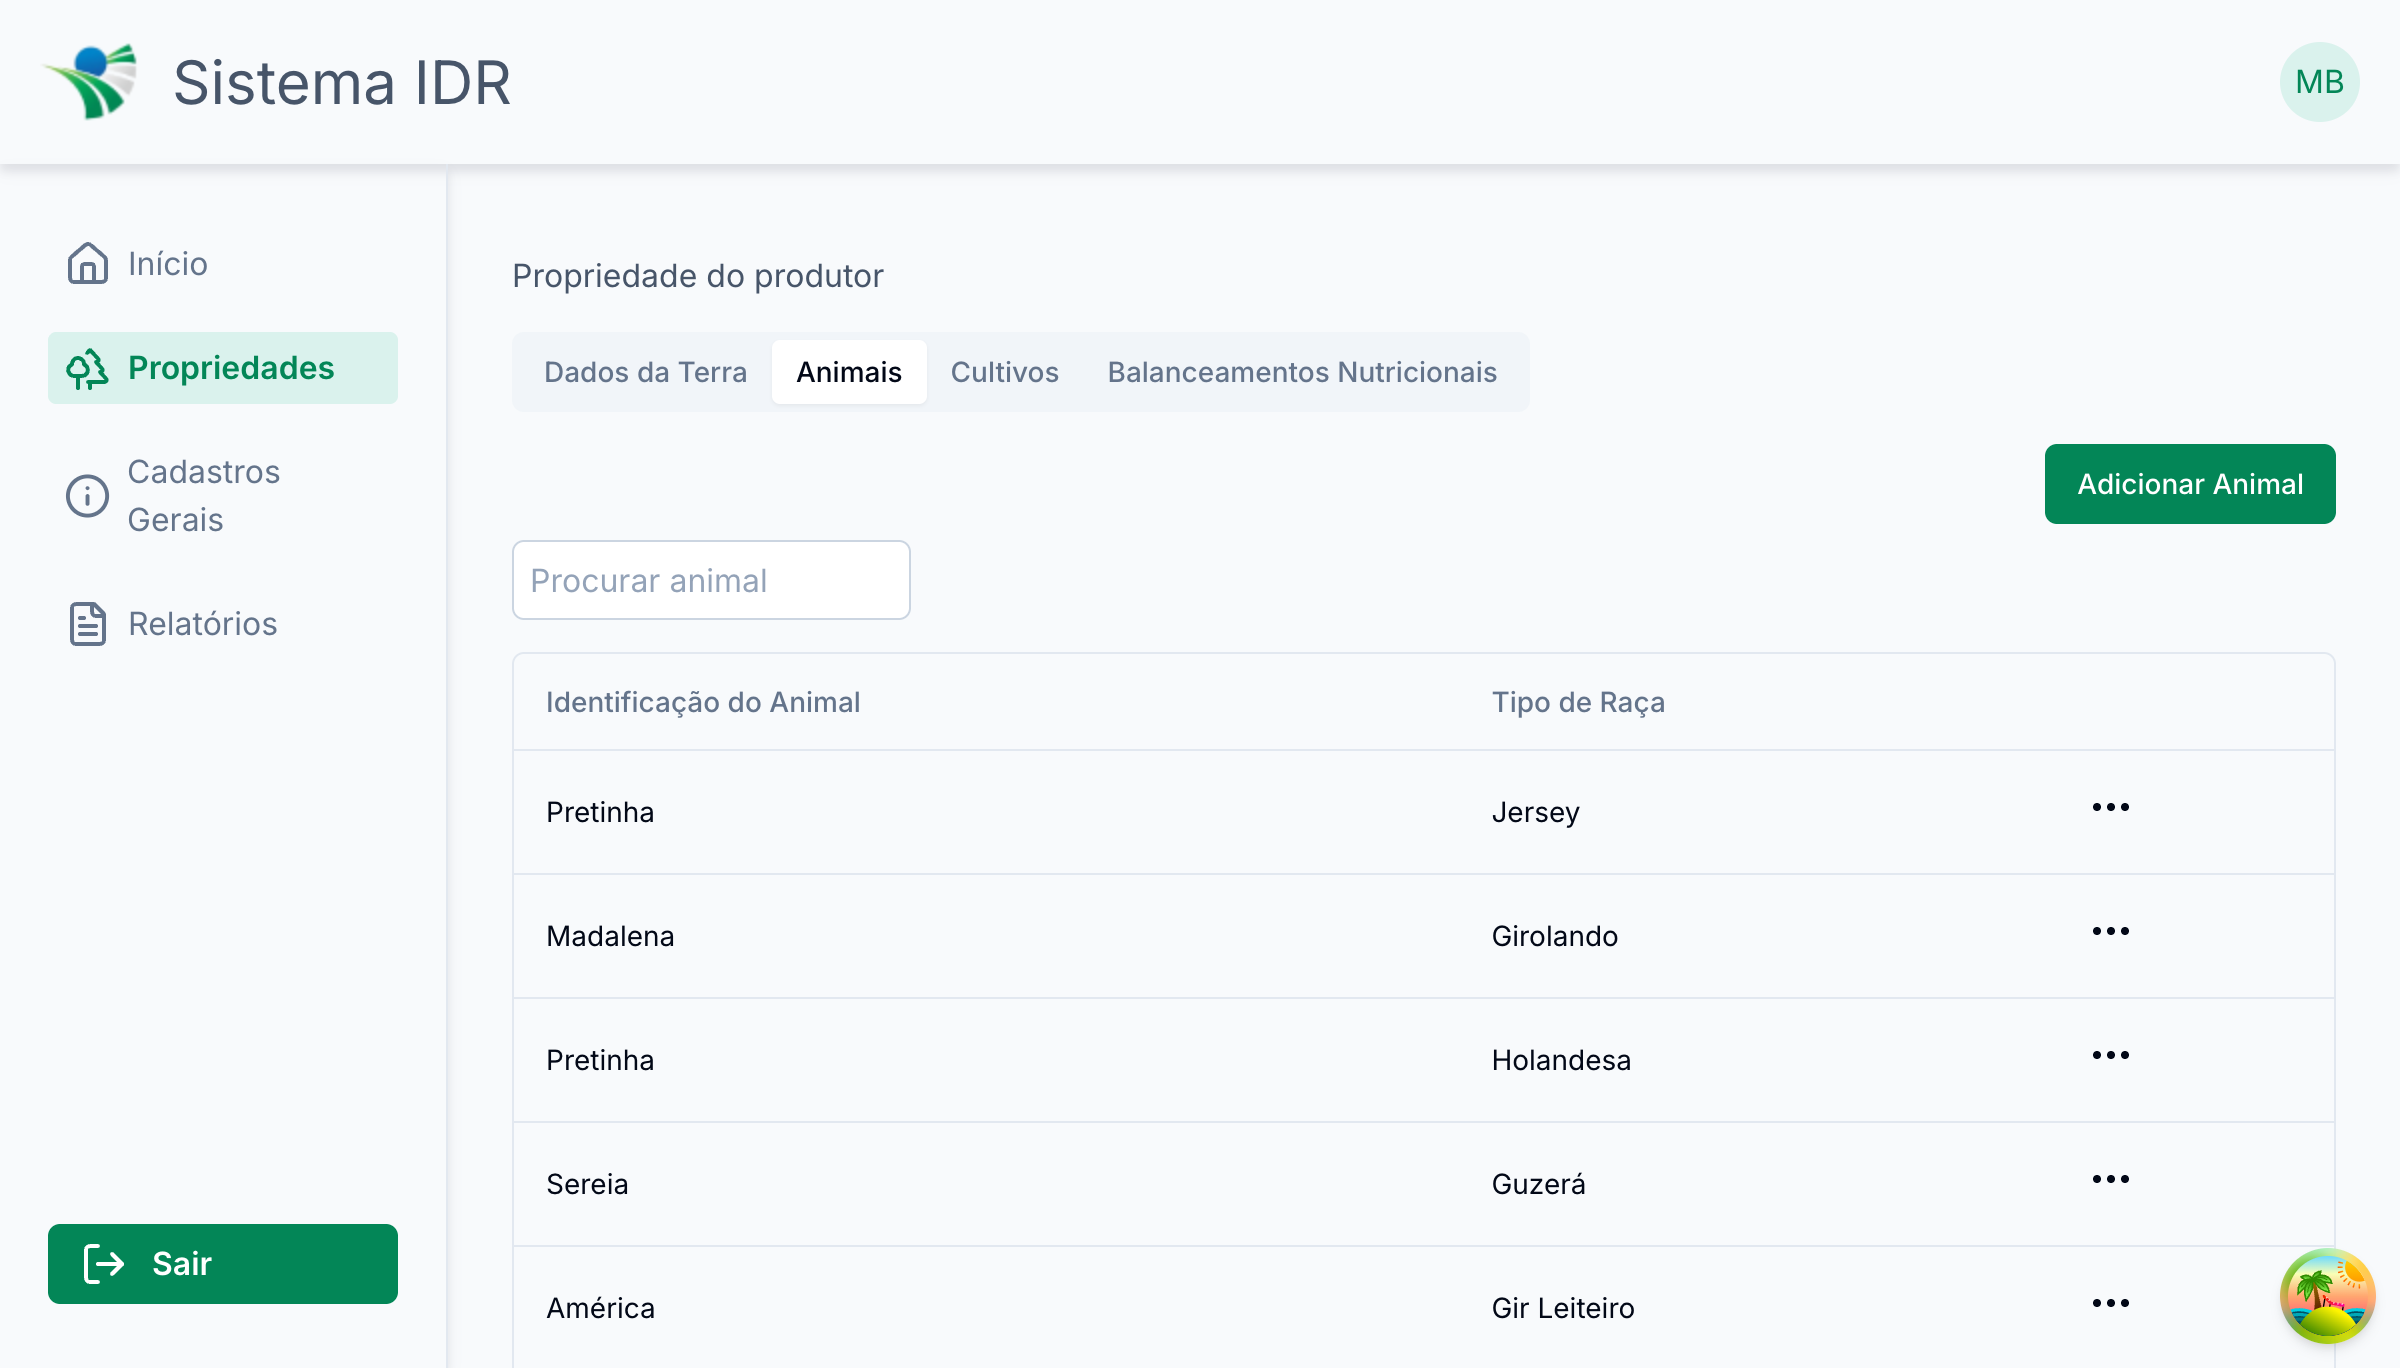
\includegraphics[width=0.8\textwidth]{figuras/sys-animais.png}
  \fonte{Autoria própria (2026)}
\end{figure}

\clearpage

Ao clicar na linha de um animal específico na listagem, o técnico acessa os detalhes clínicos e zootécnicos individuais. A tela expande-se para exibir um conjunto de subabas que representam o histórico completo do animal (\autoref{fig:sys-animal-detalhes}). Por meio dessas abas, o sistema permite a rastreabilidade abrangente de dados críticos, incluindo registros de partos, acompanhamento das fases de bezerra e novilha, diagnósticos de doenças e mastite, além do controle de entradas e saídas por meio de compras, vendas e óbitos. O sistema também permite o registro detalhado de inseminações, aplicações de medicamentos e diagnósticos de gestação.

\begin{figure}[htpb]
  \centering
  \caption{Painel de Detalhes do Animal com Subabas Modulares}
  \label{fig:sys-animal-detalhes}
  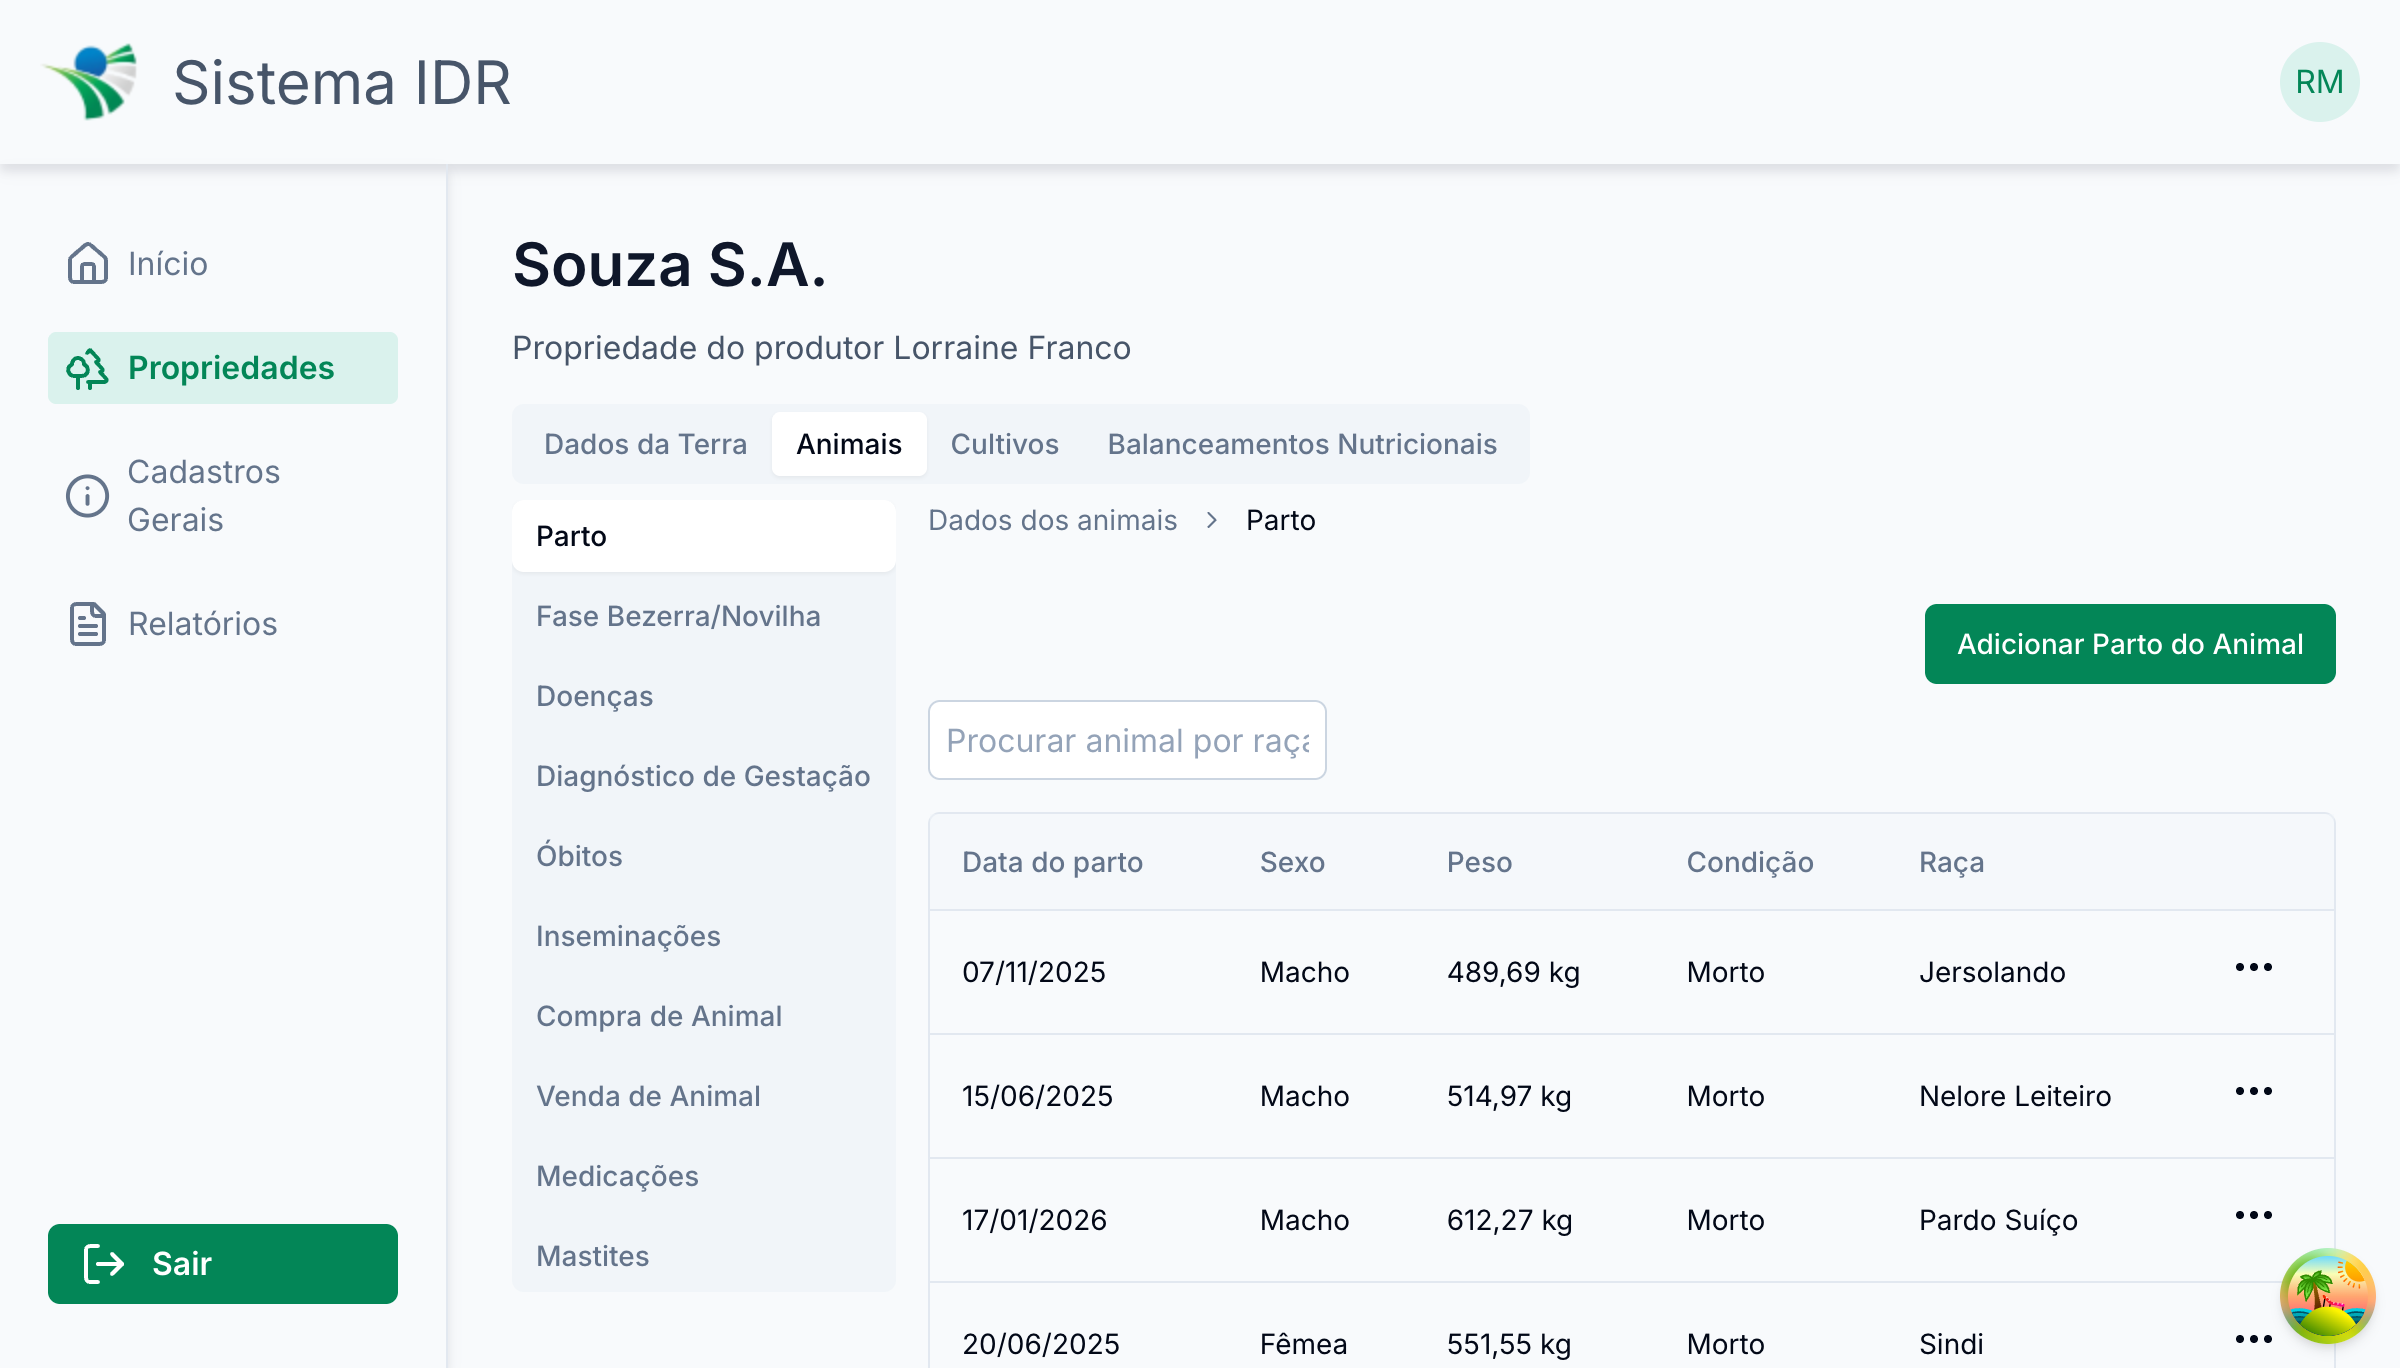
\includegraphics[width=0.8\textwidth]{figuras/sys-animal-detalhes.png}
  \fonte{Autoria própria (2026)}
\end{figure}

\clearpage

A \autoref{fig:sys-animal-submodulo} ilustra o submódulo de inseminações, que atua como um exemplo prático das diversas categorias de registros disponíveis. Neste ambiente, é possível cadastrar e consultar cada tentativa de reprodução e o status de prenhez, mantendo a rastreabilidade completa necessária para as auditorias do \gls{IDR-PR}.

\begin{figure}[htpb]
  \centering
  \caption{Submódulo de Registro de Inseminações}
  \label{fig:sys-animal-submodulo}
  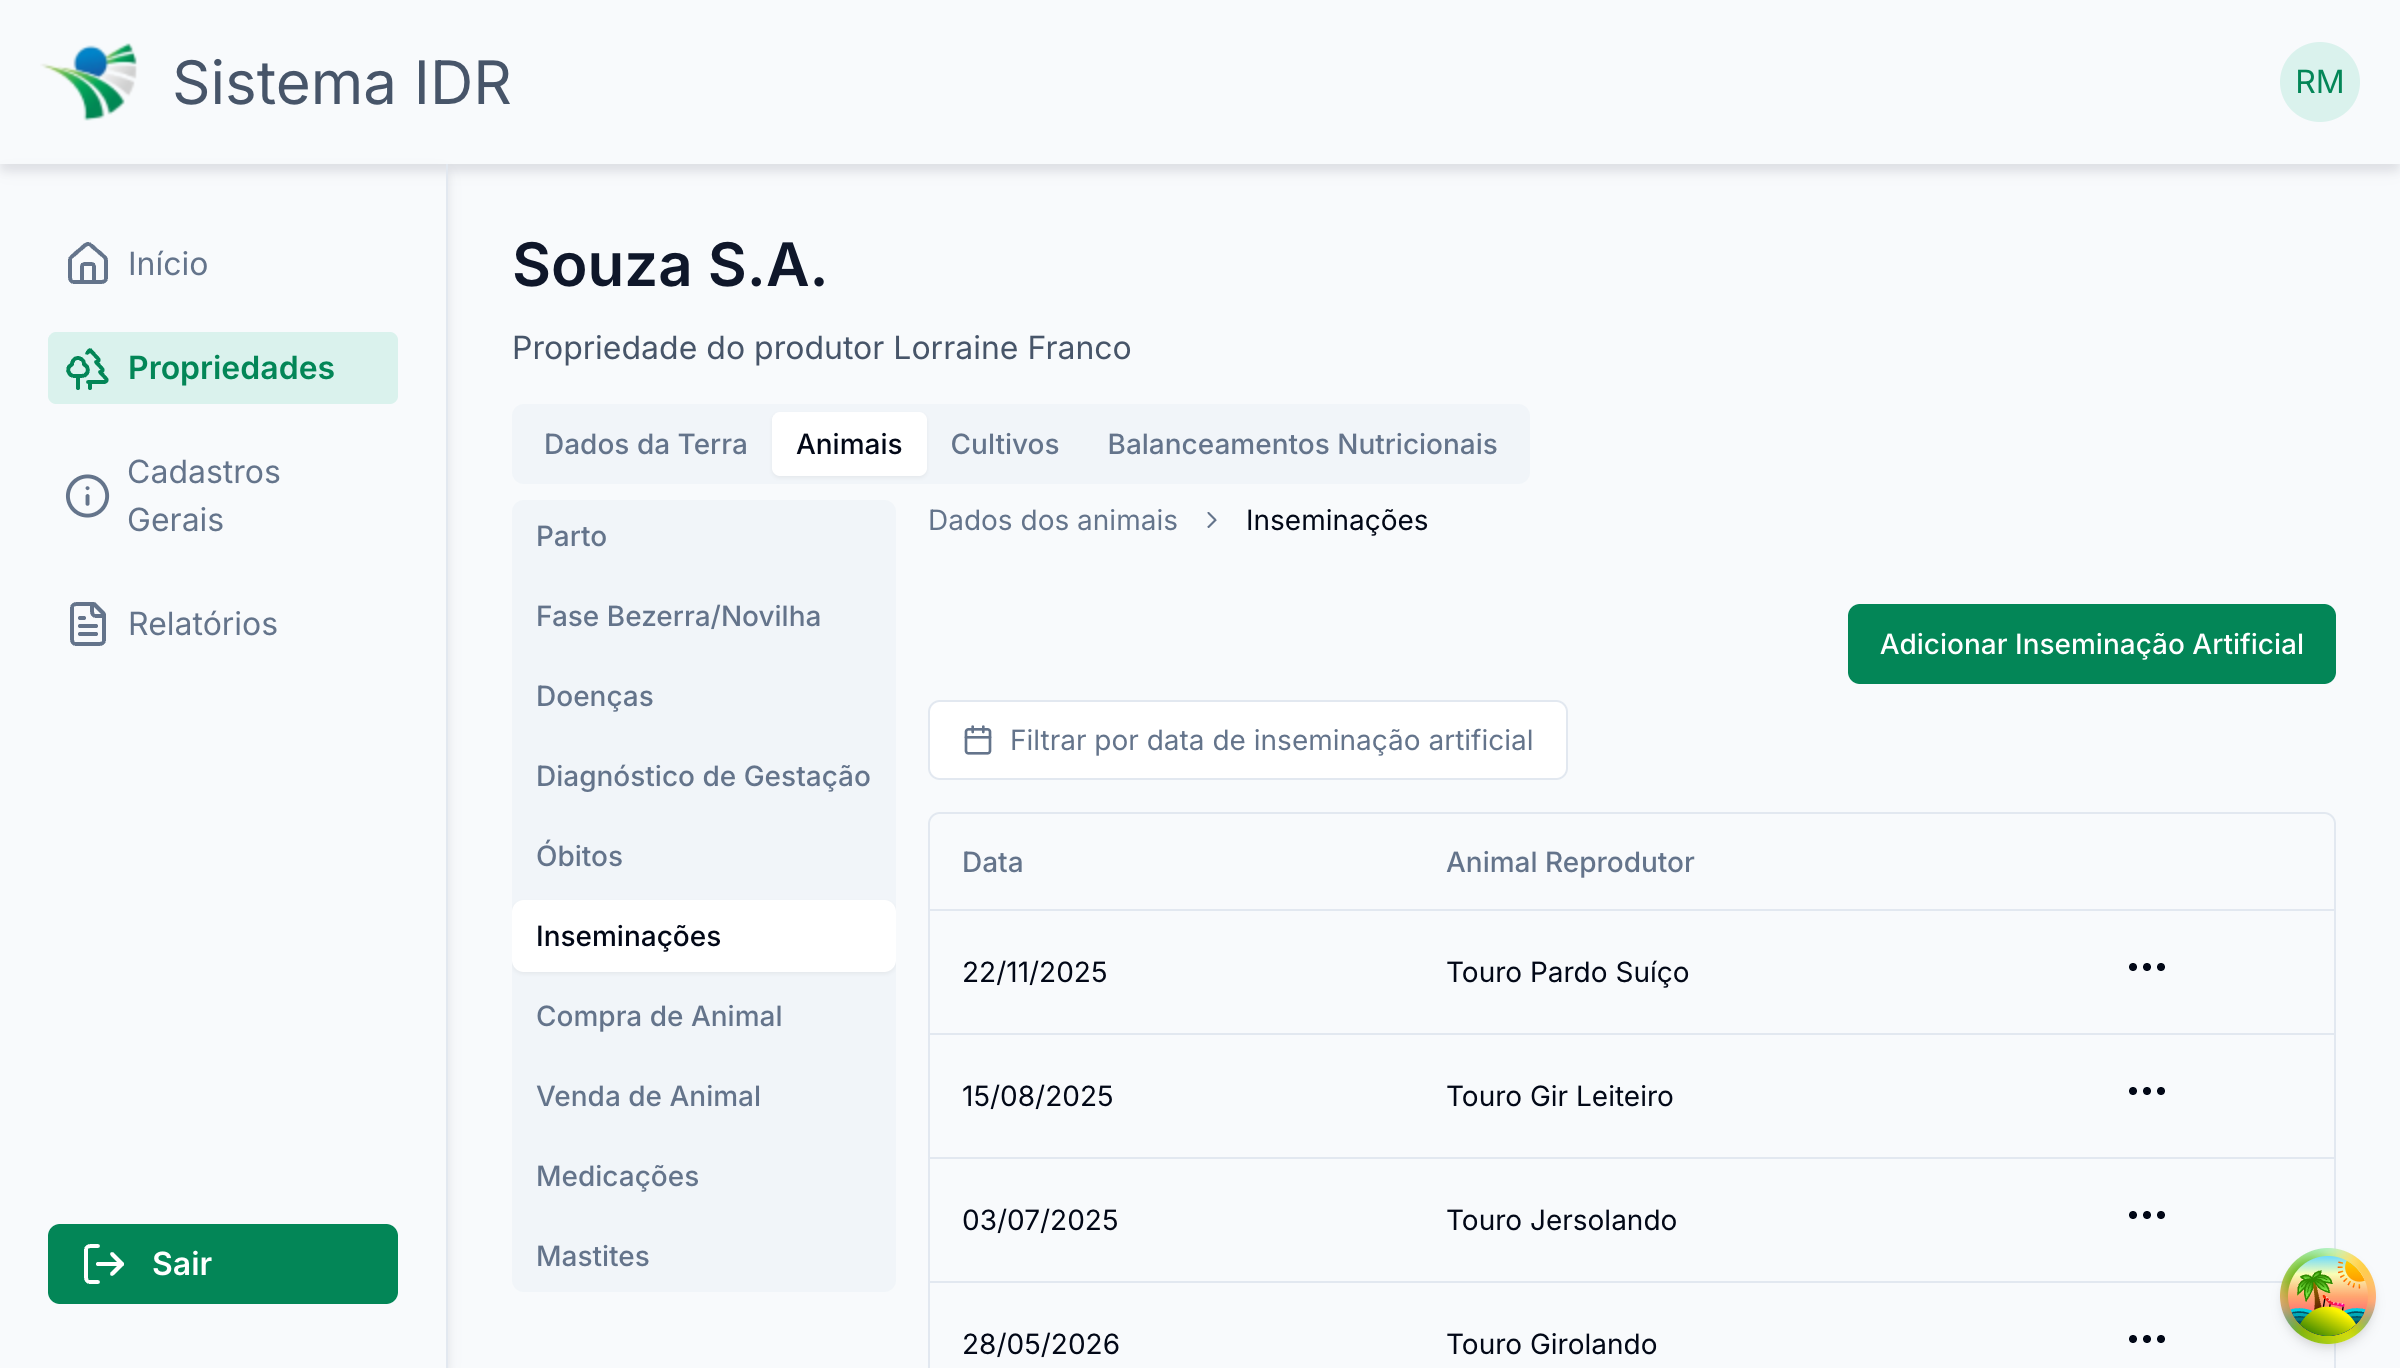
\includegraphics[width=0.8\textwidth]{figuras/sys-animal-submodulo.png}
  \fonte{Autoria própria (2026)}
\end{figure}

A arquitetura dessa interface de detalhes consolida o conceito de "prontuário único" do animal, evitando que o técnico precise navegar por diferentes páginas para entender o histórico de saúde e produção. Todos os submódulos comportam-se de maneira padronizada, integrados ao mesmo ciclo de dados e alimentando as estatísticas globais da propriedade, o que reforça a coesão do sistema perante o usuário final.

\clearpage

\subsection{Balanceamento Nutricional de Precisão}\label{subsec:apresentacaoNutricao}

A funcionalidade mais complexa do sistema é o balanceamento nutricional. A interface de Novo Balanceamento organiza-se em duas abas complementares (Visão Geral e Nutrição), sob um cabeçalho persistente que atua como suporte à navegação entre os animais da propriedade (\autoref{fig:sys-balanceamento-visao-geral-header}). Esta funcionalidade permite que o técnico alterne sequencialmente entre os animais do lote (\textit{Animal X de N}) de forma global, mantendo o contexto de navegação independentemente da sub-aba selecionada, o que garante maior agilidade operacional.

\begin{figure}[htpb]
  \centering
  \caption{Cabeçalho de Navegação Persistente no Balanceamento Nutricional}
  \label{fig:sys-balanceamento-visao-geral-header}
  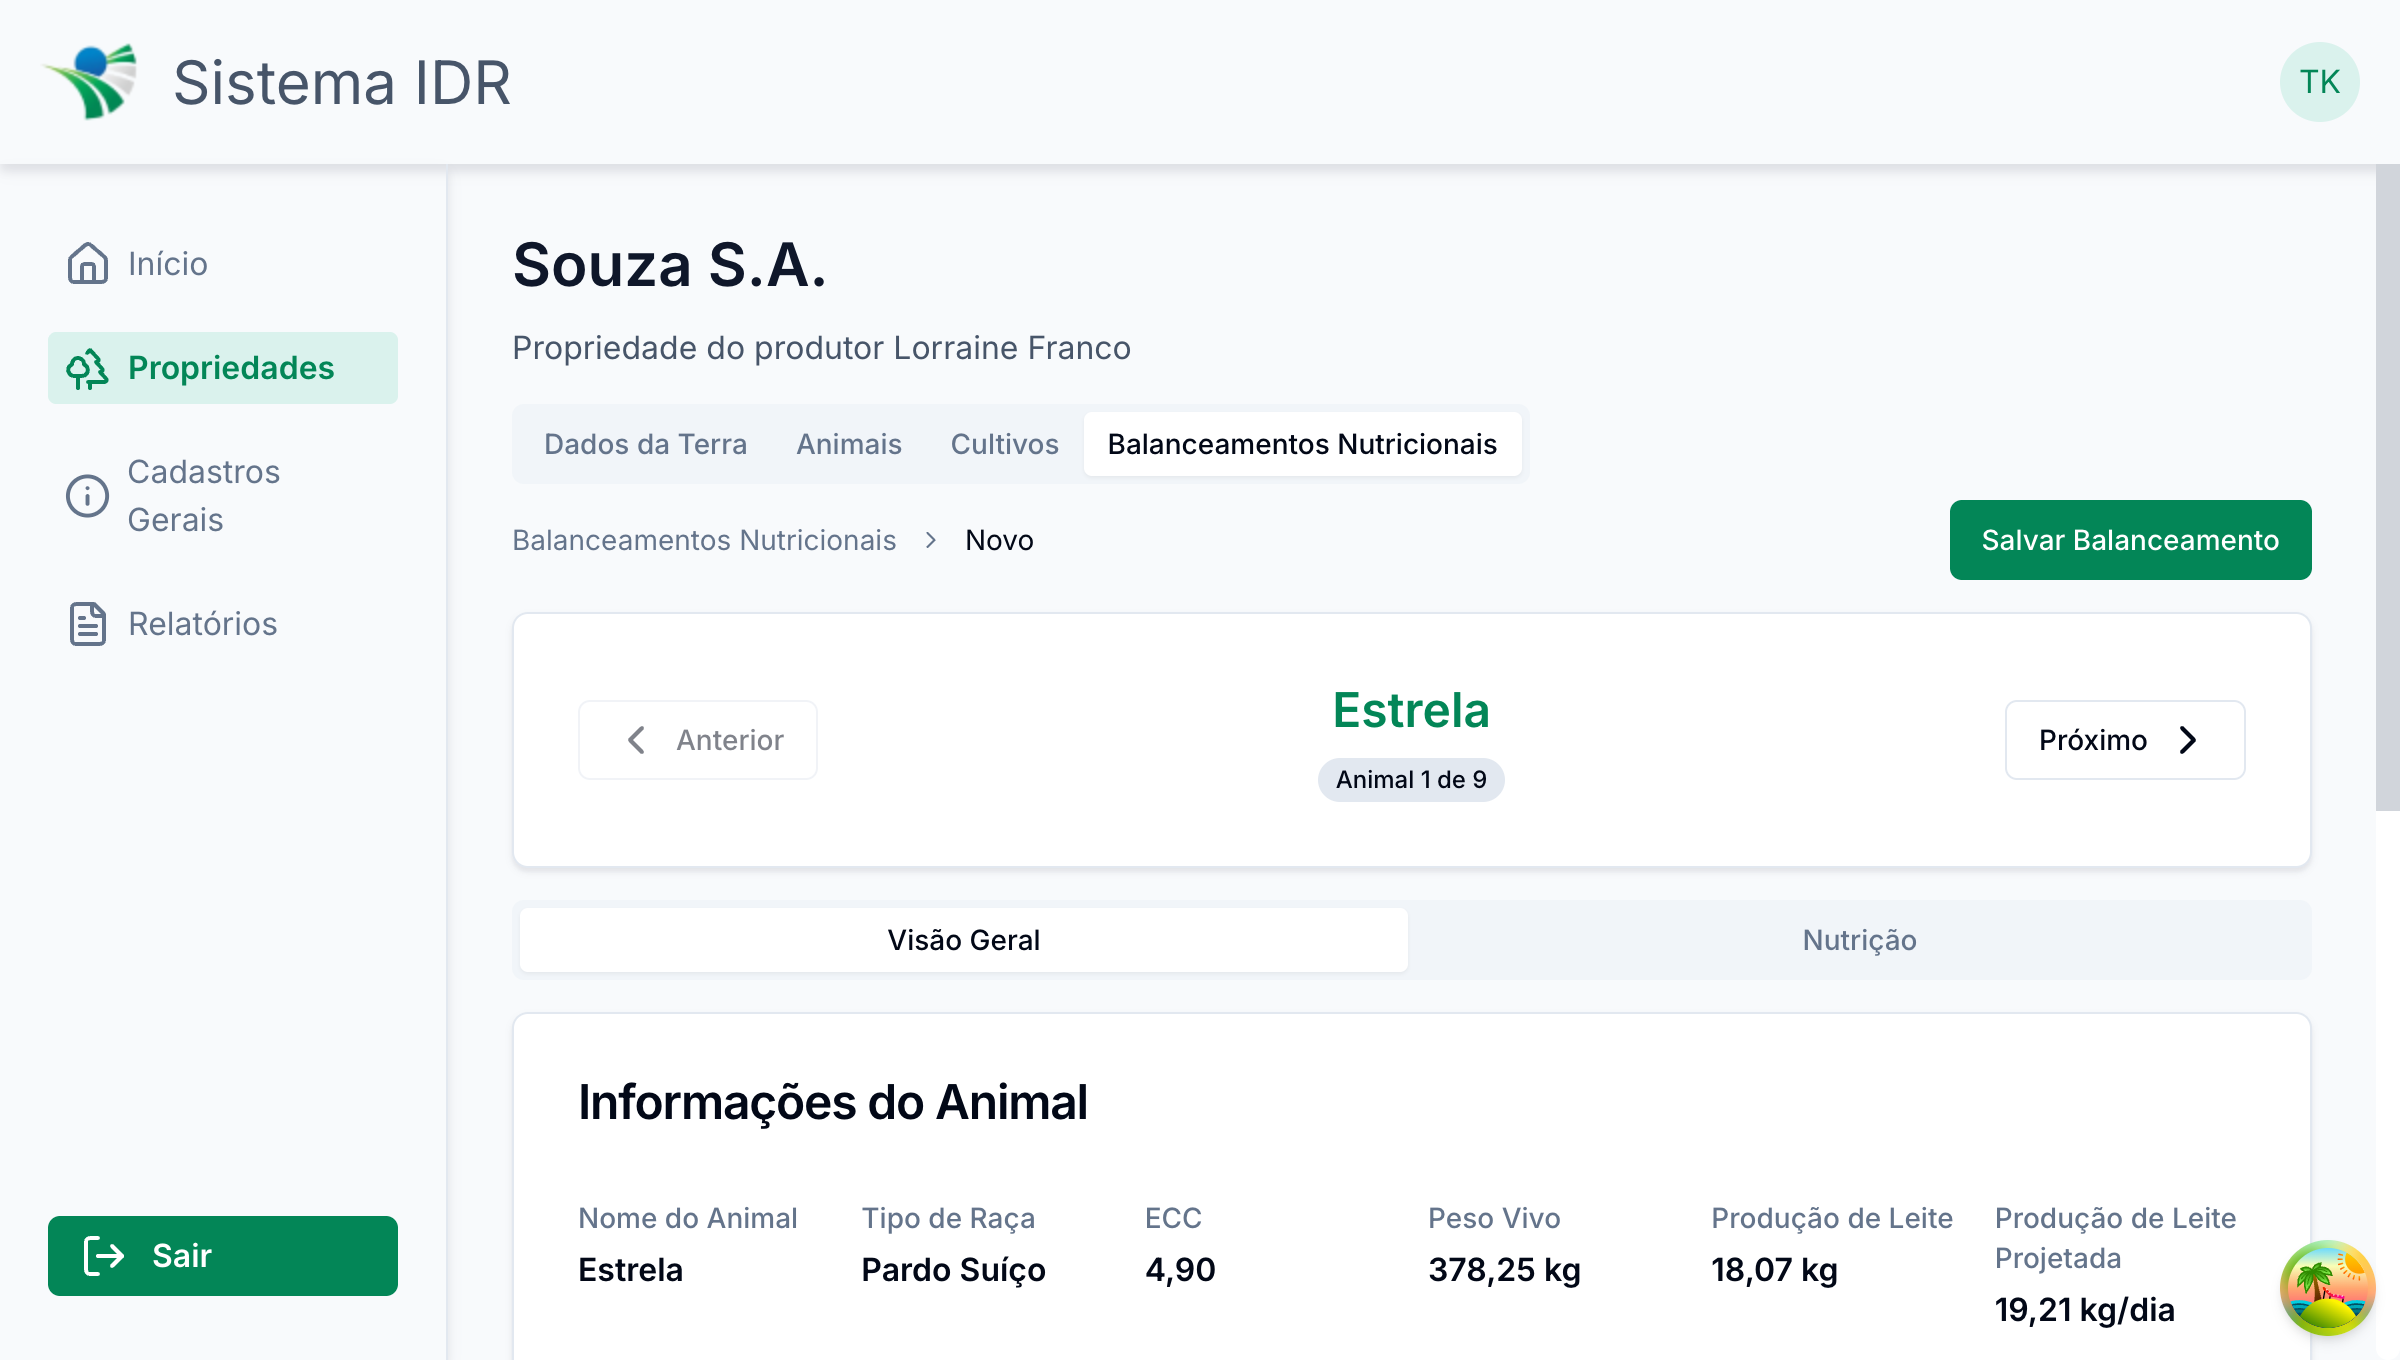
\includegraphics[width=0.8\textwidth]{figuras/sys-balanceamento-visao-geral-header.png}
  \fonte{Autoria própria (2026)}
\end{figure}

\clearpage

Na aba de Visão Geral, abaixo da navegação global, encontra-se o bloco de \textbf{Resumo Nutricional} (\autoref{fig:sys-balanceamento-visao-geral}). Este bloco exibe indicadores fundamentais do processamento da dieta, como o percentual de \gls{EE} da ração, o total de \gls{MS} consumida e as relações percentuais entre volumoso e concentrado. O sistema também calcula e apresenta a relação entre \gls{PDR} e \gls{NDT}, bem como o nível de \gls{CNF}. Esta visão garante uma análise resumida do animal em questão do rebanho.

\begin{figure}[htpb]
  \centering
  \caption{Aba de Visão Geral com Detalhamento do Resumo Nutricional}
  \label{fig:sys-balanceamento-visao-geral}
  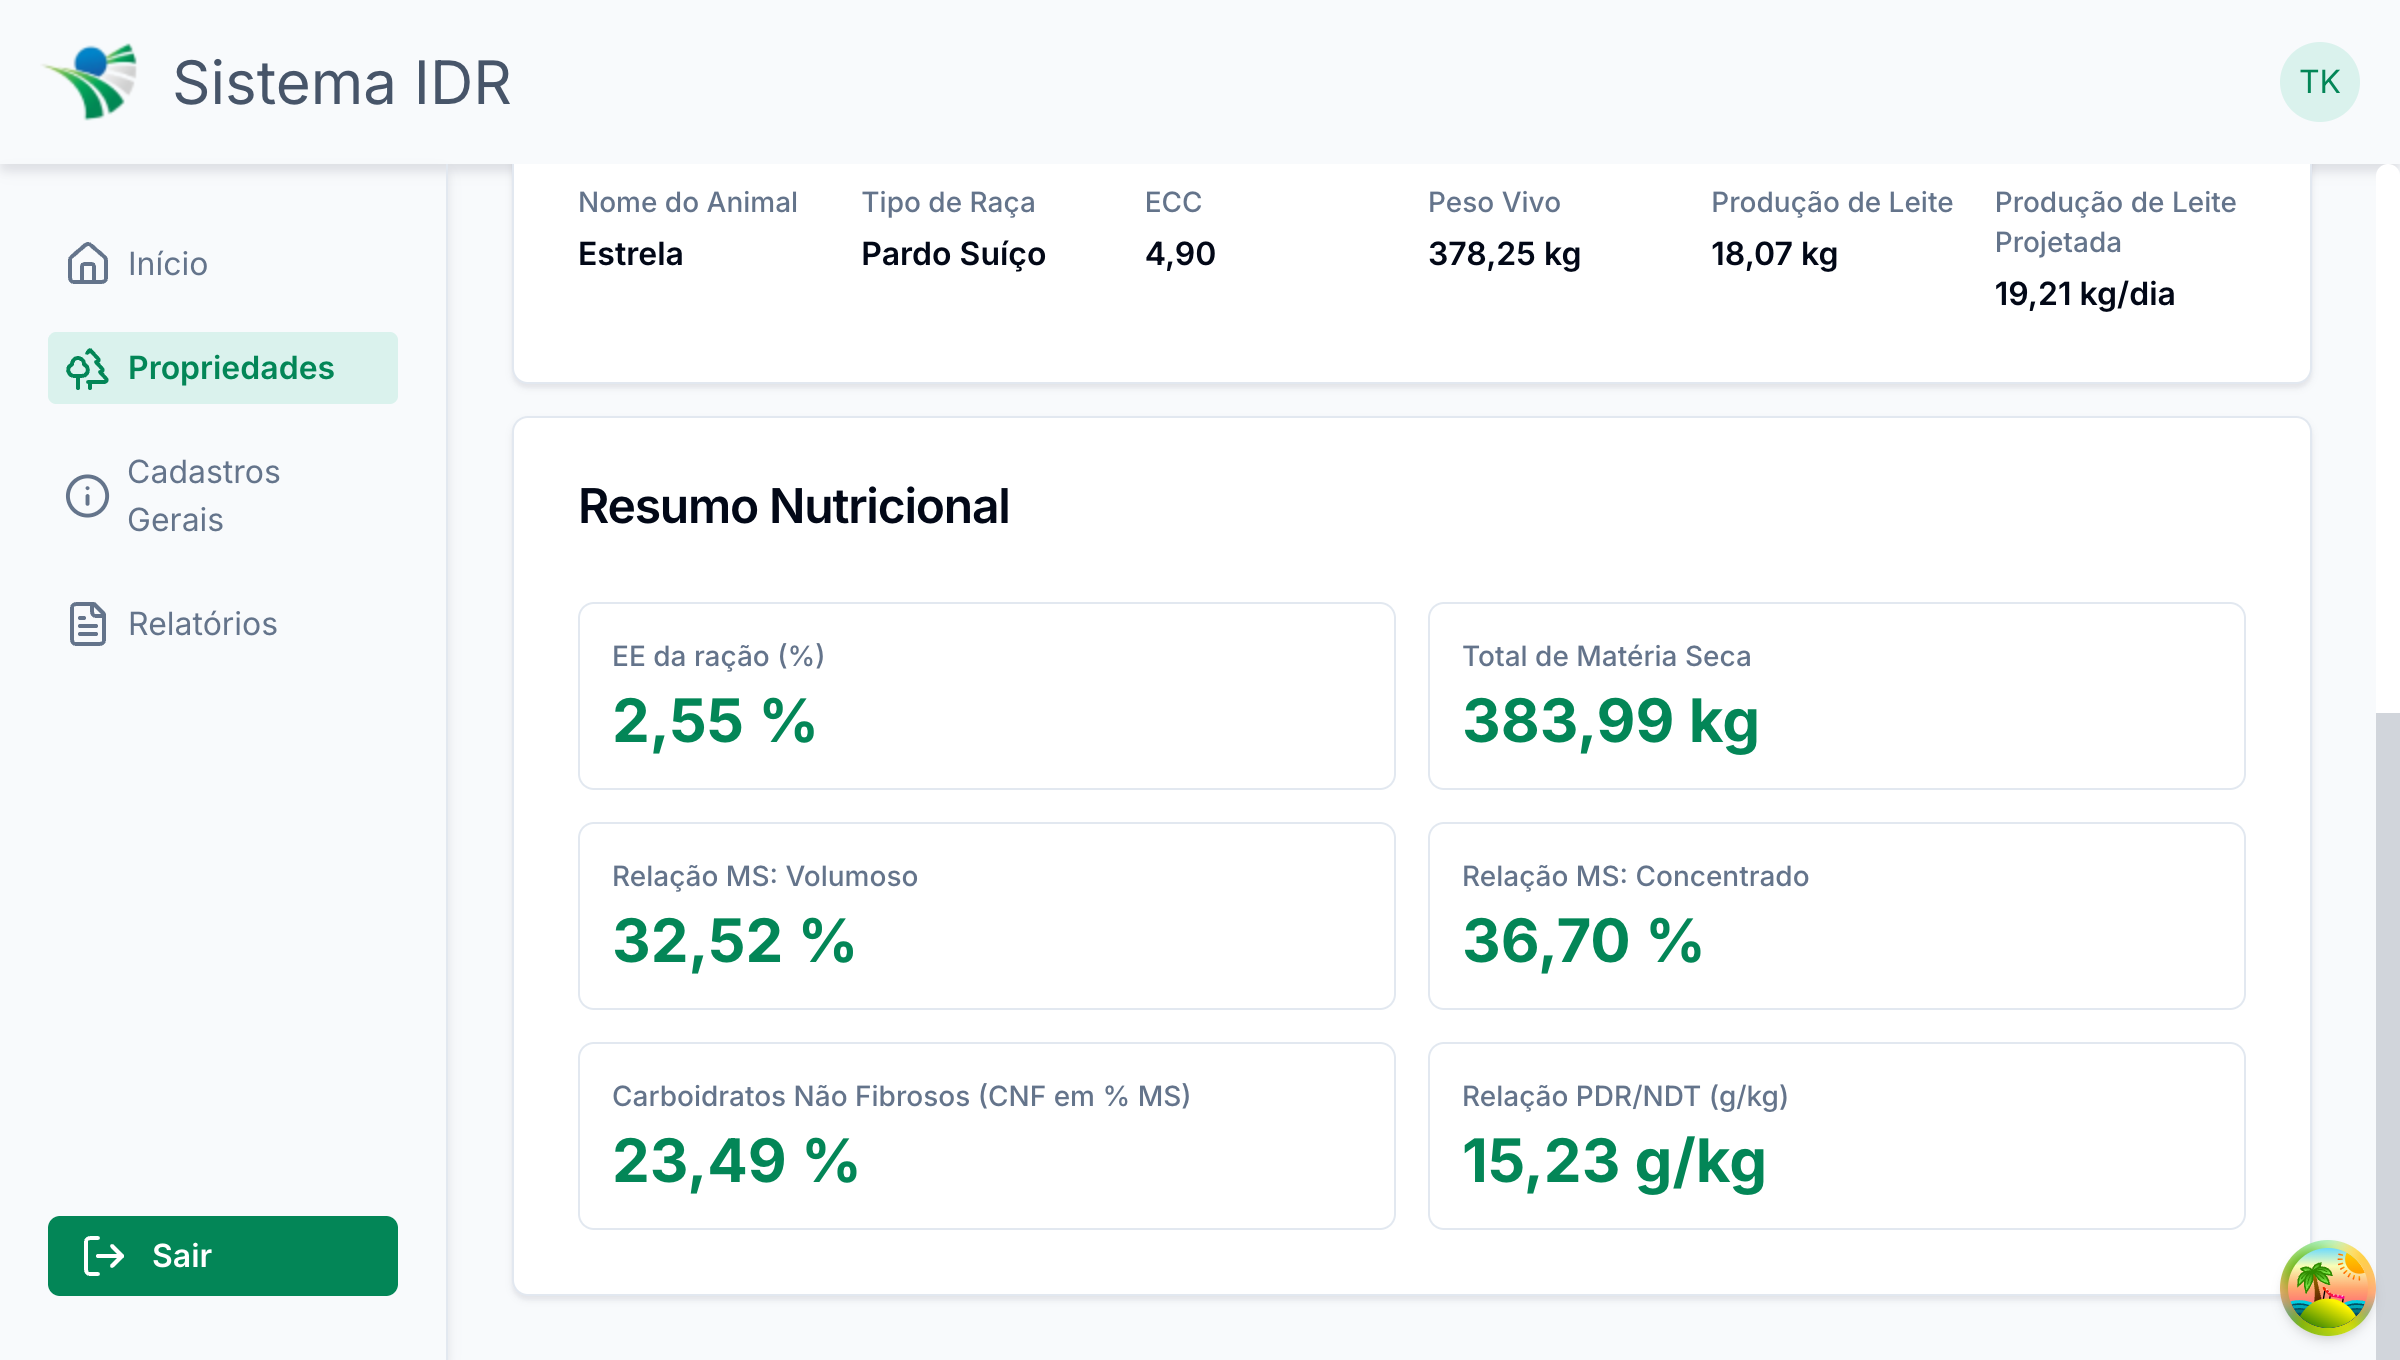
\includegraphics[width=0.8\textwidth]{figuras/sys-balanceamento-visao-geral.png}
  \fonte{Autoria própria (2026)}
\end{figure}

Na interface de Nutrição, o técnico realiza a manipulação direta da dieta. O suporte à decisão ocorre através de uma comparação visual em tempo real entre as exigências calculadas pela \gls{API} e os alimentos oferecidos. 

À medida que o técnico adiciona ou remove ingredientes via formulário (\autoref{fig:sys-balanceamento-ingrediente-form}), o sistema atualiza instantaneamente a listagem de ingredientes (\autoref{fig:sys-balanceamento-ingredientes-lista}) e os indicadores visuais de conformidade. Diferente de uma simples coleta de dados, a interface sinaliza com cores e rótulos específicos se o nutriente está em nível Normal, Acima ou Abaixo do esperado. Conforme ilustrado na \autoref{fig:sys-balanceamento-nutricao}, o sistema monitora simultaneamente múltiplos indicadores críticos, como \gls{IMS}, \gls{NDT}, \gls{PB}, \gls{Ca} e \gls{P}, garantindo que o técnico identifique desequilíbrios nutricionais de forma imediata e tome decisões informadas.

\begin{figure}[htpb]
  \centering
  \caption{Formulário para Inclusão de Ingredientes na Dieta}
  \label{fig:sys-balanceamento-ingrediente-form}
  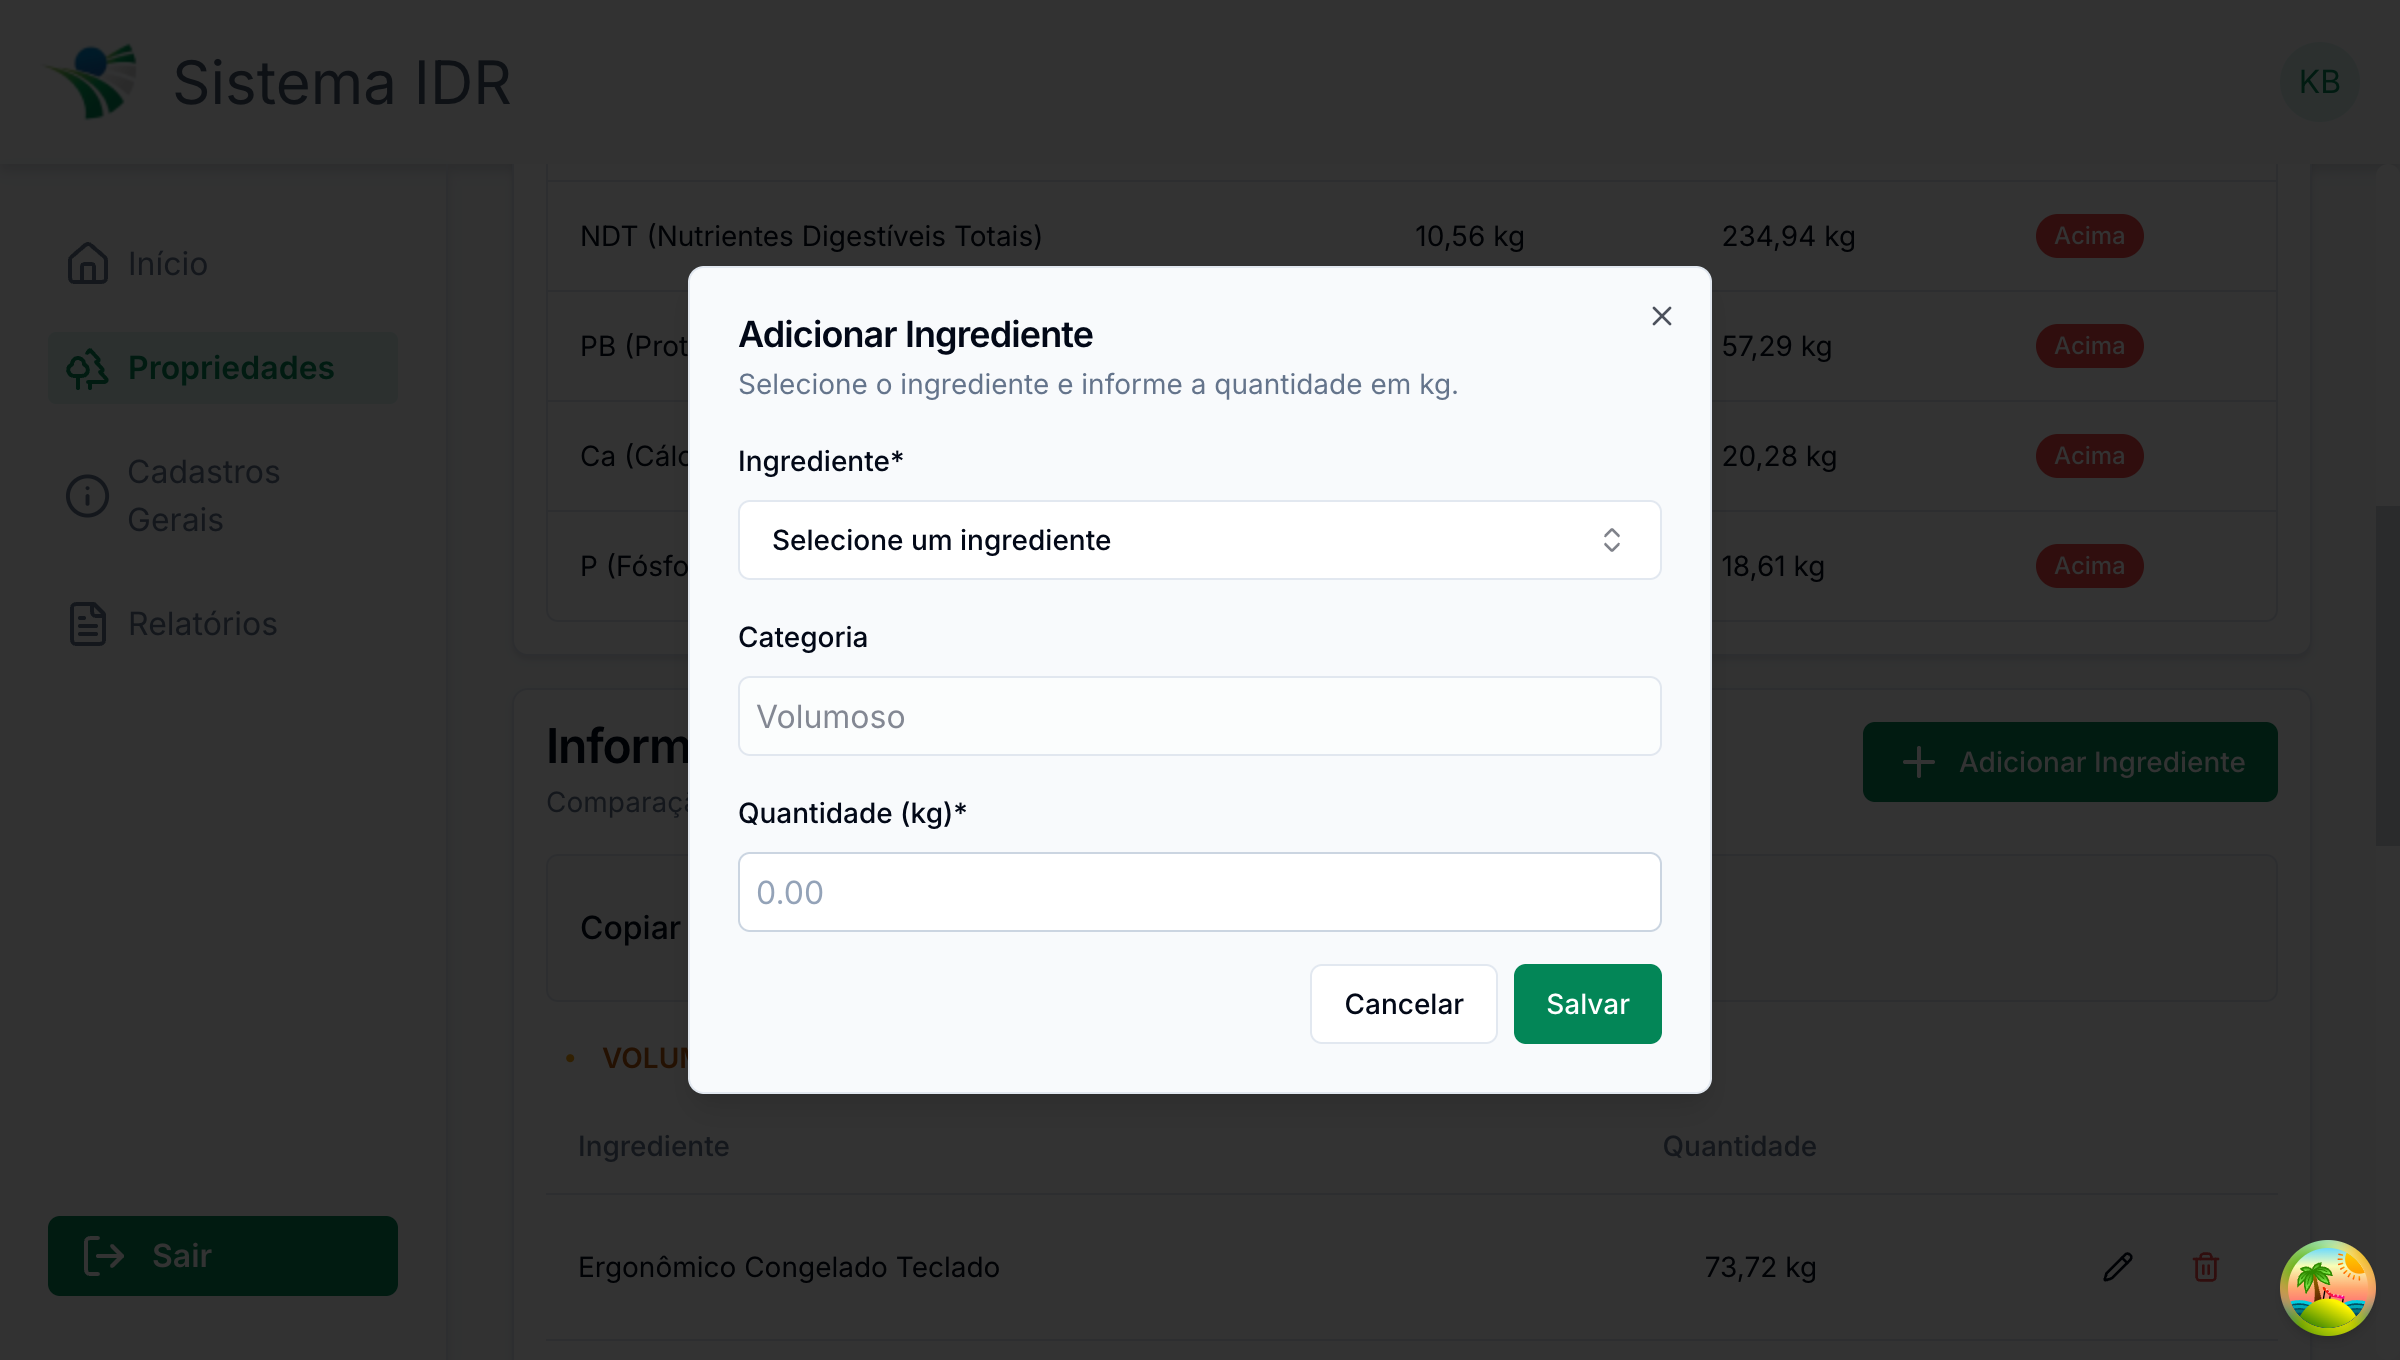
\includegraphics[width=0.6\textwidth]{figuras/sys-balanceamento-ingrediente-form.png}
  \fonte{Autoria própria (2026)}
\end{figure}

\begin{figure}[htpb]
  \centering
  \caption{Listagem de Ingredientes Oferecidos na Dieta}
  \label{fig:sys-balanceamento-ingredientes-lista}
  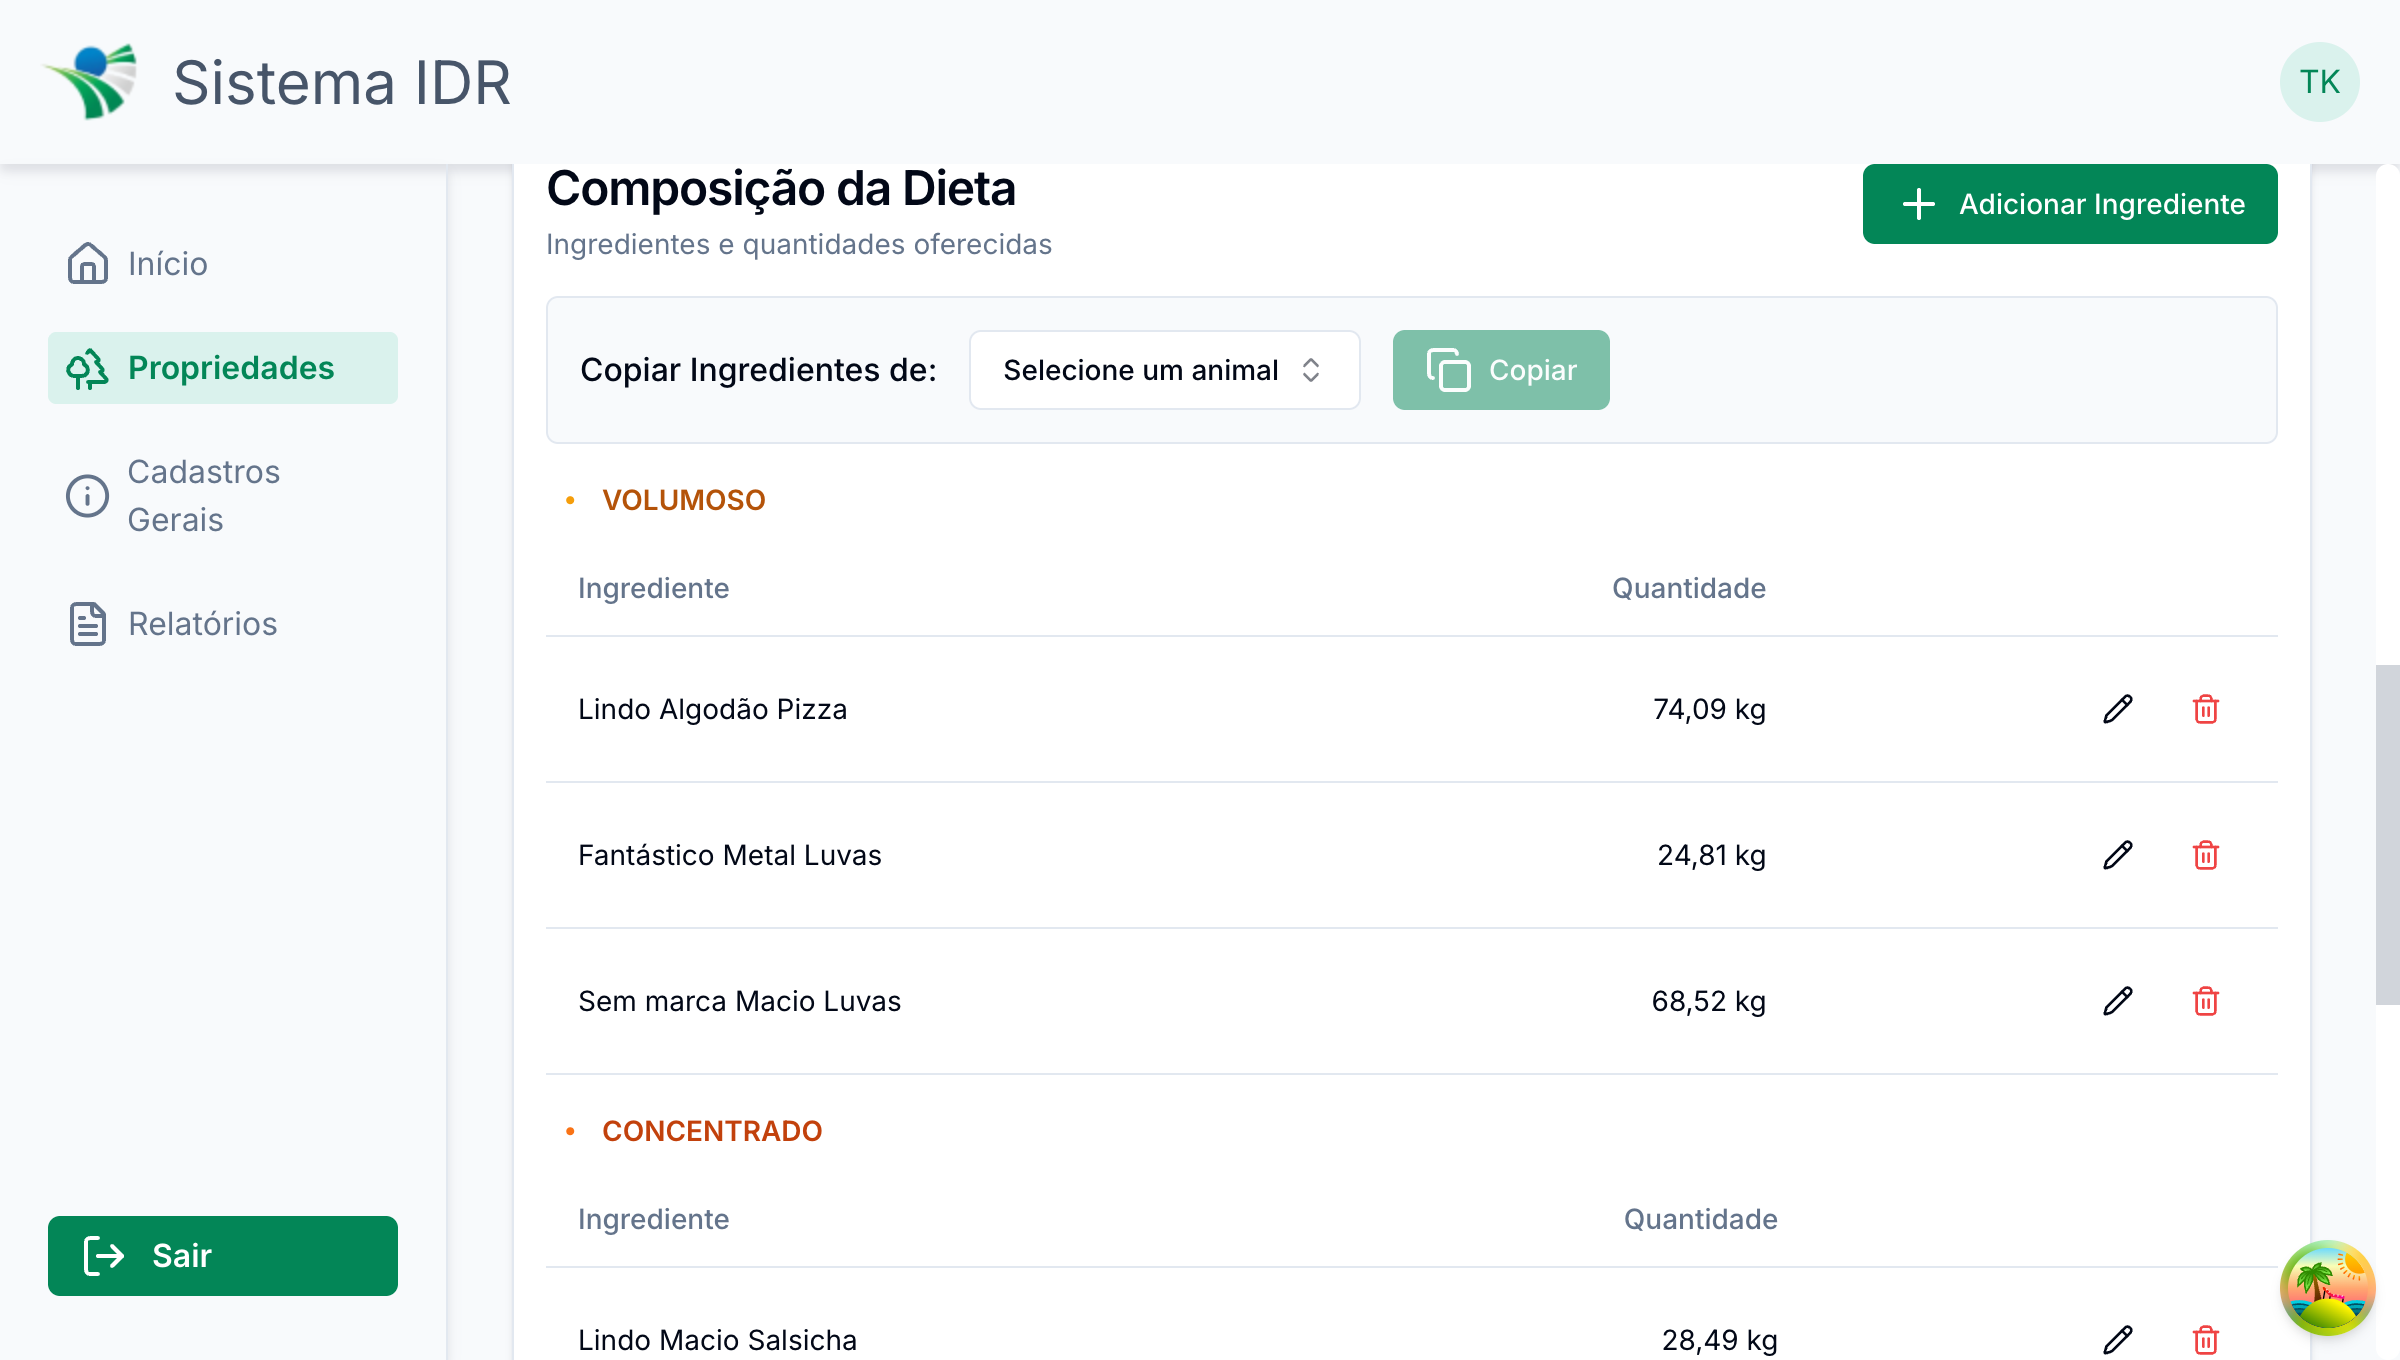
\includegraphics[width=0.8\textwidth]{figuras/sys-balanceamento-ingredientes-lista.png}
  \fonte{Autoria própria (2026)}
\end{figure}

\begin{figure}[htpb]
  \centering
  \caption{Comparação entre Exigências e Oferta com Múltiplos Indicadores de Status}
  \label{fig:sys-balanceamento-nutricao}
  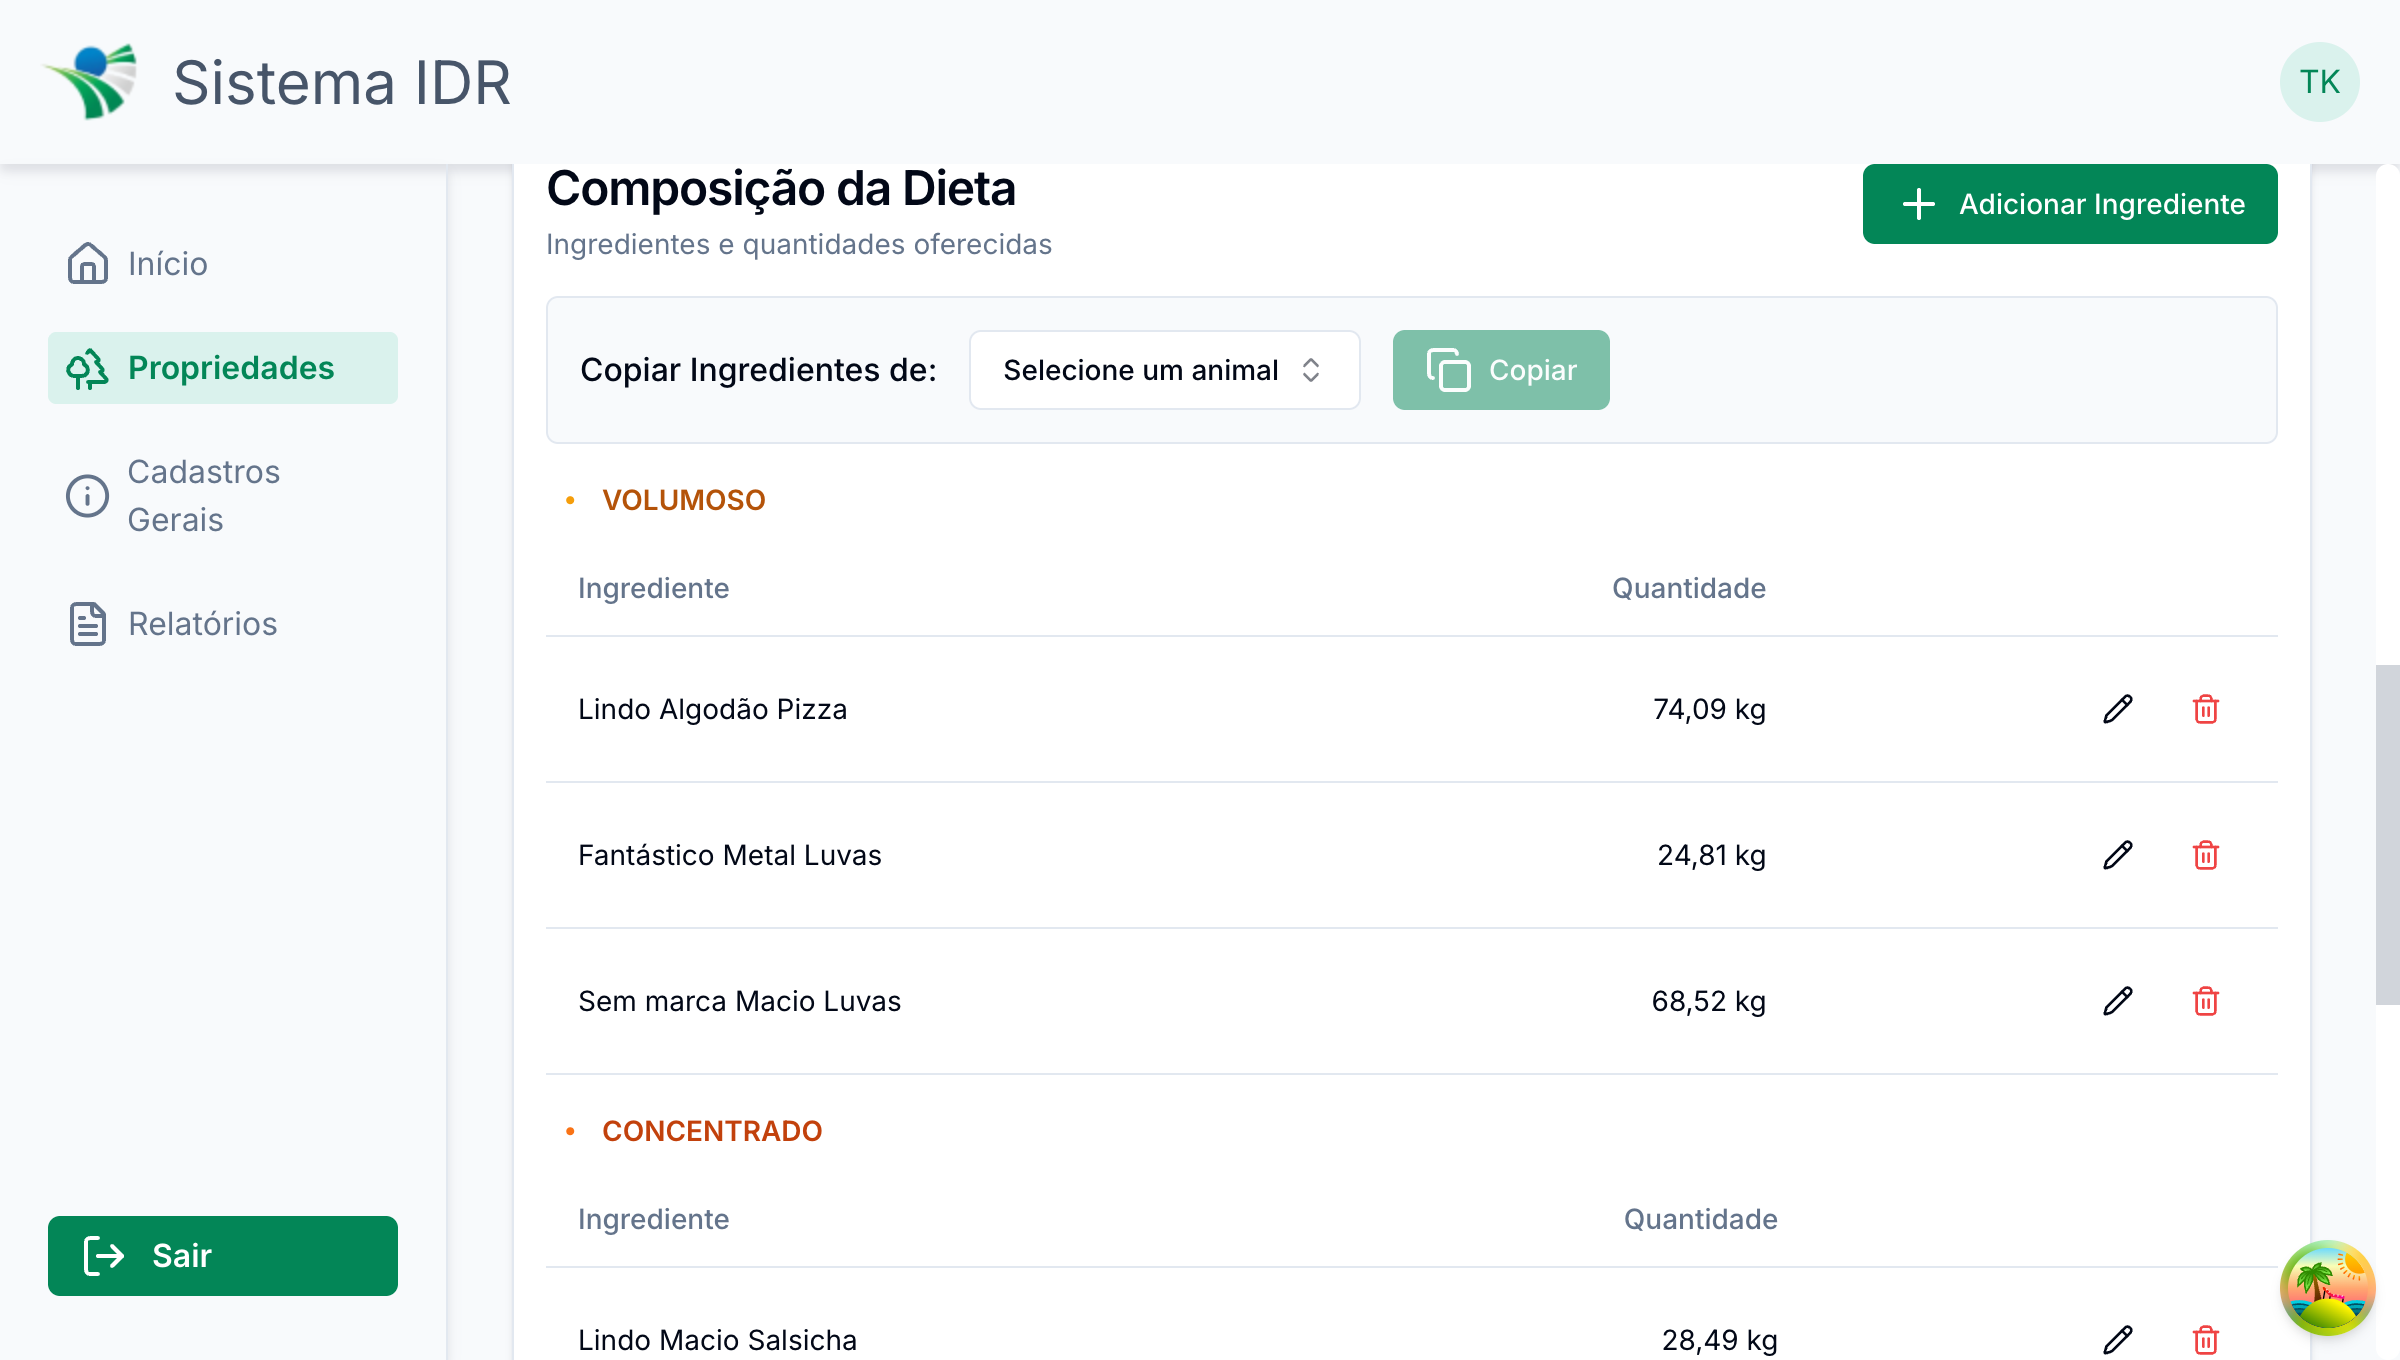
\includegraphics[width=0.8\textwidth]{figuras/sys-balanceamento-nutricao.png}
  \fonte{Autoria própria (2026)}
\end{figure}

\clearpage

Em suma, as interfaces de balanceamento nutricional transcendem a simples entrada de dados, consolidando-se como uma ferramenta estratégica de suporte à decisão. A integração entre a visualização resumida do animal e o suporte visual dinâmico durante a formulação da ração permite que o técnico execute ajustes precisos com agilidade, refletindo diretamente na eficiência produtiva e na saúde do plantel monitorado pelo \gls{IDR-PR}.

\section{Implementação do sistema}\label{sec:implementacaoSistema}

A implementação do cliente \textit{web} pautou-se na excelência técnica e no uso de padrões arquiteturais que favorecem o crescimento sustentável do software. Adotou-se o paradigma da programação reativa com a biblioteca React, utilizando TypeScript para garantir a segurança de tipos em toda a aplicação. A organização do código baseia-se em uma adaptação da \textit{Clean Architecture} dividida em diretórios independentes, focada na separação de responsabilidades.

\subsection{Infraestrutura e Configuração Base (\texttt{core})}\label{subsec:arquiteturaCore}

O diretório \texttt{core} consolida todos os protocolos globais, tipos genéricos e a infraestrutura de rede necessária. Uma das principais responsabilidades desta camada é a orquestração de requisições via contrato genérico \texttt{HttpClient}, que isola a dependência direta de bibliotecas externas como o Axios. 

Este contrato define uma estrutura única que padroniza as chamadas de comunicação para todo o sistema (\autoref{lst:http-client}). Ele engloba desde chamadas de busca individual (\textit{get one}) e de listagem (\textit{table data}), até operações de mutação como \textit{POST} (para criação), \textit{PUT} e \textit{PATCH} (para atualizações integrais ou parciais) e \textit{DELETE} (para remoções lógicas ou físicas). Ao encapsular todos esses métodos \gls{HTTP}, a camada \texttt{core} devolve os dados em um formato estritamente tipado, garantindo que módulos como o de Animais e Propriedades não precisem reescrever a lógica de integração de rede nem os tratamentos de resposta.

\begin{lstlisting}[language=TypeScript, caption={Contrato Genérico de HttpClient}, label={lst:http-client}]
export type HttpMethod = 'get' | 'post' | 'delete' | 'patch' | 'put'

export type HttpRequest<TModel = Record<string, string>, TApiModel = unknown> = {
  url: string
  method: HttpMethod
  body?: unknown
  pagination?: { page: number; perPage?: number }
  filters?: Filters<TModel>
  sort?: Sort<TModel>
  mapApiProperties?: MapApiProperties<TModel, TApiModel>
}

export type HttpClient<TModel = unknown, TApiModel = unknown, TApiResponse = TApiModel> = {
  request: (data: HttpRequest<TModel, TApiModel>) => Promise<HttpResponse<TApiResponse>>
}
\end{lstlisting}

Para conferir realismo ao ambiente de desenvolvimento, o sistema utiliza o \gls{MSW}. Além de interceptar as chamadas, implementou-se uma lógica de \textbf{simulação de atraso (\textit{delay})} nas respostas (\autoref{lst:msw-delay}), forçando a interface a lidar com estados de carregamento de forma realista.

\begin{lstlisting}[language=TypeScript, caption={Simulação de Delay Realista no \gls{MSW}}, label={lst:msw-delay}]
export function withDelay(durationMs = 1000) {
  const isTest = process.env.NODE_ENV === 'test'
  const finalDuration = isTest ? 0 : durationMs

  return (resolver: HttpResponseResolver): HttpResponseResolver =>
    async (...args) => {
      if (finalDuration > 0) await delay(finalDuration)
      return resolver(...args)
    }
}
\end{lstlisting}

Também foi desenvolvida uma lógica de \textbf{autenticação falsa (\textit{fake auth})} no \textit{middleware} do \gls{MSW} (\autoref{lst:msw-auth}), garantindo que as rotas protegidas e os cabeçalhos de autorização fossem validados antes de retornar os dados simulados.

\begin{lstlisting}[language=TypeScript, caption={Middleware de Autenticação Fake no Mock}, label={lst:msw-auth}]
export function withAuth(resolver: HttpResponseResolver): HttpResponseResolver {
  return (context) => {
    const { request } = context
    if (!request.headers.get('Authorization')) {
      return new HttpResponse(null, { status: 401 })
    }
    return resolver(context)
  }
}
\end{lstlisting}

A arquitetura do \textit{mock} reflete a modularidade do sistema. Em vez de um único arquivo monolítico, cada módulo funcional possui seus próprios \textit{handlers}. Estes são exportados de seus respectivos domínios e agrupados no arquivo central \texttt{handlers.ts} (\autoref{lst:msw-handlers}) dentro da pasta \texttt{core/mocks}, que orquestra e fornece o \textit{array} consolidado de interceptadores para o \textit{worker} inicializar a aplicação.

\begin{lstlisting}[language=TypeScript, caption={Registro Modular de Handlers no \gls{MSW}}, label={lst:msw-handlers}]
import { type HttpHandler } from 'msw'
import {
  createAnimalHandler,
  deleteAnimalHandler,
  getAnimalHandler,
  getAnimalsHandler,
  updateAnimalHandler,
} from '@/app/modules/animals/mocks/handlers/'
// Importacoes de outros modulos ocultadas para brevidade...

export const handlers: HttpHandler[] = [
  // ... handlers de autenticacao e propriedades
  createAnimalHandler,
  deleteAnimalHandler,
  getAnimalHandler,
  getAnimalsHandler,
  updateAnimalHandler,
  // ... demais handlers de todos os modulos
]
\end{lstlisting}

\subsection{Organização Modular e Estrutura de Pastas}\label{subsec:estruturaPastas}

Para manter a consistência e escalabilidade, cada módulo funcional segue uma estrutura de pastas rigorosa. A \autoref{lst:folder-structure} ilustra a organização do módulo de \textbf{Animais}, que serve como padrão para toda a aplicação. Esta separação permite que a lógica de domínio seja agnóstica à tecnologia de visualização e outras bibliotecas.

\begin{lstlisting}[caption={Estrutura de Pastas Padronizada (Módulo Animais)}, label={lst:folder-structure}]
src/app/modules/animals/
|-- domain/            # Entidades e contratos agnósticos
|   |-- models/
|   |-- use-cases/
|-- data/              # Implementação de acesso a dados e regras externas
|   |-- use-cases/
|-- main/              # Factories e injeção de dependências
|   |-- factories/
|-- mocks/             # Handlers MSW isolados por módulo
|   |-- handlers/
|-- presentation/      # Camada visual (React)
    |-- components/    # Tabelas, Dialogs de exclusão, etc.
    |-- contexts/      # Provedores de Context API
    |-- forms/         # Formulários complexos
    |-- hooks/         # Queries (TanStack) e mutações
    |-- screens/       # Telas/Páginas principais do módulo
    |-- types/         # Tipos específicos da interface
    |-- validations/   # Esquemas Zod para validação
\end{lstlisting}

\subsection{Camada de Domínio}\label{subsec:camadaDominio}

A camada de \textbf{Domain} é o ponto de partida, onde se definem as entidades e os contratos (casos de uso). Esta camada é dividida em modelos de dados (\autoref{lst:animal-models}) e definições de casos de uso (\autoref{lst:animal-use-cases}), garantindo que a regra de negócio seja expressa de forma pura, sem dependências de infraestrutura.

\begin{lstlisting}[language=TypeScript, caption={Modelos de Dados do Domínio}, label={lst:animal-models}]
export type AnimalDetailsModel = {
  name: string
  breed: Option
  weight: string
  ecc: string
  milkProduction: string
}

export type AnimalDetailsApiResponse = {
  name: string
  breed: Option
  weight: string
  ecc: string
  milkProduction: string
}

export type AnimalModel = WithId<{
  name: string
  breed: string
  weight: string
  ecc: string
  milkProduction: string
}>

export type AnimalApiResponse = AnimalModel
\end{lstlisting}

Os contratos de caso de uso padronizam como a aplicação interage com os dados de animais. A \autoref{lst:animal-use-cases} exibe o \gls{CRUD} completo, utilizando tipos genéricos para garantir a consistência de parâmetros e respostas em todas as operações.

\begin{lstlisting}[language=TypeScript, caption={Contratos de Casos de Uso (\gls{CRUD}) no Domínio}, label={lst:animal-use-cases}]
// domain/use-cases/create-animal-use-case.ts
export type CreateAnimalUseCase = RequestInterface<
  { propertyId: number; animal: AnimalDetailsModel },
  void
>

// domain/use-cases/delete-animal-use-case.ts
export type DeleteAnimalUseCase = RequestInterface<
  { propertyId: number; animalId: number },
  void
>

// domain/use-cases/get-animals-use-case.ts
export type GetAnimalsUseCase = RequestInterface<
  ListParams<AnimalModel> & { propertyId: number },
  ListResponse<AnimalModel>
>

// domain/use-cases/get-animal-use-case.ts
export type GetAnimalUseCase = RequestInterface<
  { propertyId: number; animalId: number },
  AnimalDetailsModel
>

// domain/use-cases/update-animal-use-case.ts
export type UpdateAnimalUseCase = RequestInterface<
  { propertyId: number; animal: WithId<AnimalDetailsModel> },
  void
>
\end{lstlisting}

\subsection{Camada de Dados}\label{subsec:camadaDados}

A camada de \textbf{Data} é responsável por implementar as interfaces definidas no domínio, comunicando-se com serviços externos ou \gls{API}s. Todos os casos de uso do domínio possuem suas respectivas classes \texttt{Remote} na camada de dados. A \autoref{lst:animal-data} ilustra como essas implementações utilizam o \texttt{HttpClient} para realizar requisições de rede e tratam as respostas e erros, mapeando-os para exceções de negócio compreensíveis.

\begin{lstlisting}[language=TypeScript, caption={Implementações da Camada Data (\gls{CRUD})}, label={lst:animal-data}]
// data/use-cases/remote-create-animal-use-case.ts
export class RemoteCreateAnimalUseCase implements CreateAnimalUseCase {
  constructor(
    private readonly url: string,
    private readonly httpClient: HttpClient
  ) {}

  execute: CreateAnimalUseCase['execute'] = async ({ propertyId, animal }) => {
    const url = this.url.replace(':propertyId', String(propertyId))

    const { statusCode } = await this.httpClient.request({
      url,
      method: 'post',
      body: animal,
    })

    if (statusCode === HttpStatusCode.created) return

    if (statusCode === HttpStatusCode.badRequest) throw new BadRequestError()

    if (statusCode === HttpStatusCode.forbidden) {
      throw new ForbiddenError(
        'Você não tem permissão para criar um novo animal'
      )
    }

    throw new UnexpectedError()
  }
}

// data/use-cases/remote-delete-animal-use-case.ts
export class RemoteDeleteAnimalUseCase implements DeleteAnimalUseCase {
  constructor(
    private readonly url: string,
    private readonly httpClient: HttpClient
  ) {}

  execute: DeleteAnimalUseCase['execute'] = async ({
    propertyId,
    animalId,
  }) => {
    const url = this.url.replace(':propertyId', String(propertyId))

    const { statusCode } = await this.httpClient.request({
      url: `${url}/${animalId}`,
      method: 'delete',
    })

    if (statusCode === HttpStatusCode.noContent) return

    if (statusCode === HttpStatusCode.notFound) {
      throw new NotFoundError('Animal')
    }

    if (statusCode === HttpStatusCode.forbidden) {
      throw new ForbiddenError('Você não tem permissão para excluir um animal')
    }

    throw new UnexpectedError()
  }
}

// data/use-cases/remote-get-animal-use-case.ts
export class RemoteGetAnimalUseCase implements GetAnimalUseCase {
  constructor(
    private readonly url: string,
    private readonly httpClient: HttpClient<
      AnimalDetailsModel,
      AnimalDetailsApiResponse
    >
  ) {}

  execute: GetAnimalUseCase['execute'] = async ({ animalId, propertyId }) => {
    const url = this.url.replace(':propertyId', String(propertyId))

    const { statusCode, body } = await this.httpClient.request({
      url: `${url}/${animalId}`,
      method: 'get',
    })

    if (statusCode === HttpStatusCode.ok && !!body) {
      return {
        name: body.name,
        breed: body.breed,
        ecc: body.ecc,
        weight: body.weight,
        milkProduction: body.milkProduction,
      }
    }

    if (statusCode === HttpStatusCode.notFound)
      throw new NotFoundError('Animal')

    if (statusCode === HttpStatusCode.forbidden) {
      throw new ForbiddenError('Você não tem permissão para buscar um animal')
    }

    throw new UnexpectedError()
  }
}

// data/use-cases/remote-get-animals-use-case.ts
export class RemoteGetAnimalsUseCase implements GetAnimalsUseCase {
  constructor(
    private readonly url: string,
    private readonly httpClient: HttpClient<
      AnimalModel,
      AnimalApiResponse,
      ListApiResponse<AnimalApiResponse[]>
    >
  ) {}

  execute: GetAnimalsUseCase['execute'] = async ({
    propertyId,
    filters,
    pagination,
    sort,
  }) => {
    const mapApiProperties: MapApiProperties<AnimalModel, AnimalApiResponse> = {
      id: 'id',
      name: 'name',
      breed: 'breed',
      ecc: 'ecc',
      weight: 'weight',
      milkProduction: 'milkProduction',
    }

    const url = this.url.replace(':propertyId', String(propertyId))

    const { statusCode, body } = await this.httpClient.request({
      url: `${url}/search`,
      method: 'post',
      filters,
      pagination,
      sort,
      mapApiProperties,
    })

    if (statusCode === HttpStatusCode.ok && !!body) {
      return {
        resources: body.content.map((item) => ({
          id: item.id,
          name: item.name,
          breed: item.breed,
          weight: item.weight,
          ecc: item.ecc,
          milkProduction: item.milkProduction,
        })),
        totalPages: Math.ceil(body.numberOfElements / body.pageable.pageSize),
      }
    }

    if (statusCode === HttpStatusCode.notFound) {
      throw new NotFoundError('Animais')
    }

    if (statusCode === HttpStatusCode.forbidden) {
      throw new ForbiddenError('Você não tem permissão para buscar os animais')
    }

    throw new UnexpectedError()
  }
}

// data/use-cases/remote-update-animal-use-case.ts
export class RemoteUpdateAnimalUseCase implements UpdateAnimalUseCase {
  constructor(
    private readonly url: string,
    private readonly httpClient: HttpClient
  ) {}

  execute: UpdateAnimalUseCase['execute'] = async ({
    propertyId,
    animal: { id, ...animal },
  }) => {
    const url = this.url.replace(':propertyId', String(propertyId))

    const { statusCode } = await this.httpClient.request({
      url: `${url}/${id}`,
      method: 'patch',
      body: animal,
    })

    if (statusCode === HttpStatusCode.noContent) return

    if (statusCode === HttpStatusCode.badRequest) throw new BadRequestError()

    if (statusCode === HttpStatusCode.forbidden) {
      throw new ForbiddenError('Você não tem permissão para editar um animal')
    }

    throw new UnexpectedError()
  }
}
\end{lstlisting}

\subsection{Camada Main (Fábricas)}\label{subsec:camadaMain}

A camada \textbf{Main} atua como \textit{Composition Root}, utilizando o padrão \textit{Factory} para instanciar as classes da camada \textit{Data} injetando as dependências necessárias. Essa abordagem protege a interface gráfica de precisar conhecer detalhes de infraestrutura, como o cliente \gls{HTTP} ou \gls{URL}s específicas da \gls{API}. A \autoref{lst:animal-main} ilustra as fábricas de todo o ciclo de vida de dados do módulo.

\begin{lstlisting}[language=TypeScript, caption={Fábricas de Injeção de Dependências}, label={lst:animal-main}]
// main/factories/use-cases/remote-create-animal-use-case-factory.ts
export function makeRemoteCreateAnimalUseCase(): CreateAnimalUseCase {
  return new RemoteCreateAnimalUseCase(
    'properties/:propertyId/animals',
    makeApiHttpClient()
  )
}

// main/factories/use-cases/remote-delete-animal-use-case-factory.ts
export function makeRemoteDeleteAnimalUseCase(): DeleteAnimalUseCase {
  return new RemoteDeleteAnimalUseCase(
    'properties/:propertyId/animals',
    makeApiHttpClient()
  )
}

// main/factories/use-cases/remote-get-animal-use-case-factory.ts
export function makeRemoteGetAnimalUseCase(): GetAnimalUseCase {
  return new RemoteGetAnimalUseCase(
    'properties/:propertyId/animals',
    makeApiHttpClient<AnimalDetailsModel, AnimalDetailsApiResponse>()
  )
}

// main/factories/use-cases/remote-get-animals-use-case-factory.ts
export function makeRemoteGetAnimalsUseCase(): GetAnimalsUseCase {
  return new RemoteGetAnimalsUseCase(
    'properties/:propertyId/animals',
    makeApiHttpClient<
      AnimalModel,
      AnimalApiResponse,
      ListApiResponse<AnimalApiResponse[]>
    >()
  )
}

// main/factories/use-cases/remote-update-animal-use-case-factory.ts
export function makeRemoteUpdateAnimalUseCase(): UpdateAnimalUseCase {
  return new RemoteUpdateAnimalUseCase(
    'properties/:propertyId/animals',
    makeApiHttpClient()
  )
}
\end{lstlisting}

\subsection{Camada de Mocks}\label{subsec:camadaMocks}

A camada de \textbf{Mocks} é fundamental para a agilidade no desenvolvimento. Ela contém os \textit{handlers} do \gls{MSW} que interceptam especificamente as rotas deste módulo (\autoref{lst:animal-mock}). Isso permite simular o comportamento completo da \gls{API} oficial, mantendo um estado interno persistente durante a sessão para permitir testes reais de criação, edição e exclusão sem depender do \textit{backend}.

\begin{lstlisting}[language=TypeScript, caption={Handlers \gls{MSW} para Simulação de \gls{API}}, label={lst:animal-mock}]
// mocks/handlers/create-animal-handler.ts
export const createAnimalHandler = httpWithMiddleware<
  PathParams<'propertyId'>,
  AnimalDetailsModel,
  never
>({
  routePath: '/api/properties/:propertyId/animals',
  method: 'post',
  middlewares: [withDelay(), withAuth],
  resolver: async () =>
    HttpResponse.json({}, { status: HttpStatusCode.created }),
})

// mocks/handlers/delete-animal-handler.ts
export const deleteAnimalHandler = httpWithMiddleware<
  PathParams<'propertyId' | 'id'>,
  never,
  never
>({
  routePath: '/api/properties/:propertyId/animals/:id',
  method: 'delete',
  middlewares: [withDelay(), withAuth],
  resolver: async () =>
    HttpResponse.json(undefined, {
      status: 204,
    }),
})

// mocks/handlers/get-animal-handler.ts
export const getAnimalHandler = httpWithMiddleware<
  PathParams<'propertyId' | 'id'>,
  never,
  AnimalDetailsApiResponse
>({
  routePath: '/api/properties/:propertyId/animals/:id',
  method: 'get',
  middlewares: [withDelay(), withAuth],
  resolver: async ({ params }) => {
    if (!animalsData.length) {
      return HttpResponse.json({} as AnimalDetailsApiResponse, {
        status: 404,
      })
    }

    const animalFound = animalsData.find(
      (animal) => animal.id === Number(params.id)
    )

    if (!animalFound) {
      return HttpResponse.json({} as AnimalDetailsApiResponse, {
        status: 404,
      })
    }

    return HttpResponse.json(
      {
        name: animalFound.name,
        breed: {
          label: animalFound.breed,
          value: faker.number.int({ min: 1, max: 1000 }),
        },
        ecc: animalFound.ecc,
        milkProduction: animalFound.milkProduction,
        weight: animalFound.weight,
      },
      { status: HttpStatusCode.ok }
    )
  },
})

// mocks/handlers/get-animals-handler.ts
export const getAnimalsHandler = httpWithMiddleware<
  PathParams<'propertyId'>,
  MockParams<AnimalApiResponse>,
  MockResponse<AnimalApiResponse[]>
>({
  routePath: '/api/properties/:propertyId/animals/search',
  method: 'post',
  middlewares: [withDelay(), withAuth],
  resolver: async ({ request }) => {
    const { filters, page, rows, sort } = await request.json()

    if (!animalsData.length) {
      return HttpResponse.json(
        {
          content: [],
          numberOfElements: 0,
          pageable: {
            pageSize: 0,
          },
        },
        {
          status: 404,
        }
      )
    }

    let animals = animalsData as AnimalApiResponse[]

    if (filters) animals = filterData<AnimalApiResponse>(filters, animals)
    if (sort) animals = sortData<AnimalApiResponse>(sort, animals)
    const numberOfElements = animals.length
    animals = paginateData<AnimalApiResponse>({ page, perPage: rows }, animals)

    return HttpResponse.json(
      {
        content: animals,
        numberOfElements,
        pageable: {
          pageSize: rows,
        },
      },
      { status: HttpStatusCode.ok }
    )
  },
})

// mocks/handlers/update-animal-handler.ts
export const updateAnimalHandler = httpWithMiddleware<
  PathParams<'propertyId' | 'id'>,
  never,
  never
>({
  routePath: '/api/properties/:propertyId/animals/:id',
  method: 'patch',
  middlewares: [withDelay(), withAuth],
  resolver: async () =>
    HttpResponse.json(undefined, { status: HttpStatusCode.noContent }),
})
\end{lstlisting}

\subsection{Camada de Apresentação (Presentation)}\label{subsec:camadaApresentacao}

A camada de \textbf{Presentation} é o ponto de convergência que materializa as regras de negócio em uma interface interativa. Esta camada é subdividida em subdiretórios que isolam responsabilidades de estado, interface e validação:

\begin{itemize}
    \item \texttt{contexts/}: Gerenciamento de estado global do módulo via Context API.
    \item \texttt{hooks/}: Encapsulamento de lógicas complexas e consultas ao TanStack Query.
    \item \texttt{components/}: Partes visuais isoladas (ex: Tabela de Animais).
    \item \texttt{forms/} e \texttt{validations/}: Lógica de preenchimento e esquemas Zod.
    \item \texttt{screens/}: Orquestração final das páginas do módulo.
    \item \texttt{types/}: Definições de tipos exclusivas para a interface.
\end{itemize}

O fluxo de dados se inicia pelo \textbf{Contexto} (\autoref{lst:animal-context}), que centraliza informações como o identificador da propriedade e o animal selecionado, provendo funções de controle para abertura de formulários e diálogos, eliminando a necessidade de repasse manual de propriedades (\textit{prop drilling}).

\begin{lstlisting}[language=TypeScript, caption={Gerenciamento de Estado no Context \gls{API}}, label={lst:animal-context}]
type AnimalContextValue = {
  propertyId: number
  filters: AnimalFilters
  handleChangeFilters: (newFilters: AnimalFilters) => void
  selectedAnimal?: AnimalModel
  isOpenNewAnimalForm: boolean
  isOpenEditAnimalForm: boolean
  isOpenDeleteAnimalContainer: boolean
  openNewAnimalForm: () => void
  closeNewAnimalForm: () => void
  openEditAnimalForm: (animal: AnimalModel) => void
  closeEditAnimalForm: () => void
  openDeleteAnimalContainer: (animal: AnimalModel) => void
  closeDeleteAnimalContainer: () => void
}

export const AnimalContext = createContext<AnimalContextValue>(
  {} as AnimalContextValue
)

export function AnimalProvider({ children }: Readonly<PropsWithChildren>) {
  const params = useParams<{ propertyId: string }>()

  const [filters, setFilters] = useState<AnimalFilters>({})

  const handleChangeFilters = useCallback((newFilters: AnimalFilters) => {
    setFilters((prevState) => ({
      ...prevState,
      ...newFilters,
    }))
  }, [])

  const [isOpenNewAnimalForm, setIsOpenNewAnimalForm] = useState(false)

  const [isOpenEditAnimalForm, setIsOpenEditAnimalForm] = useState(false)

  const [isOpenDeleteAnimalContainer, setIsOpenDeleteAnimalContainer] =
    useState(false)

  const [selectedAnimal, setSelectedAnimal] = useState<AnimalModel>()

  const openNewAnimalForm = useCallback(() => {
    setIsOpenNewAnimalForm(true)
  }, [])

  const closeNewAnimalForm = useCallback(() => {
    setIsOpenNewAnimalForm(false)
  }, [])

  const openEditAnimalForm = useCallback((animal: AnimalModel) => {
    setSelectedAnimal(animal)
    setIsOpenEditAnimalForm(true)
  }, [])

  const closeEditAnimalForm = useCallback(() => {
    setSelectedAnimal(undefined)
    setIsOpenEditAnimalForm(false)
  }, [])

  const openDeleteAnimalContainer = useCallback((animal: AnimalModel) => {
    setSelectedAnimal(animal)
    setIsOpenDeleteAnimalContainer(true)
  }, [])

  const closeDeleteAnimalContainer = useCallback(() => {
    setSelectedAnimal(undefined)
    setIsOpenDeleteAnimalContainer(false)
  }, [])

  const providerValues = useMemo(
    () => ({
      propertyId: Number(params.propertyId),
      filters,
      handleChangeFilters,
      selectedAnimal,
      isOpenNewAnimalForm,
      isOpenEditAnimalForm,
      isOpenDeleteAnimalContainer,
      openNewAnimalForm,
      closeNewAnimalForm,
      openEditAnimalForm,
      closeEditAnimalForm,
      openDeleteAnimalContainer,
      closeDeleteAnimalContainer,
    }),
    [
      params.propertyId,
      filters,
      handleChangeFilters,
      selectedAnimal,
      isOpenNewAnimalForm,
      isOpenEditAnimalForm,
      isOpenDeleteAnimalContainer,
      openNewAnimalForm,
      closeNewAnimalForm,
      openEditAnimalForm,
      closeEditAnimalForm,
      openDeleteAnimalContainer,
      closeDeleteAnimalContainer,
    ]
  )

  if (!params.propertyId) {
    return null
  }

  return (
    <AnimalContext.Provider value={providerValues}>
      {children}
    </AnimalContext.Provider>
  )
}
\end{lstlisting}

Os \textbf{Hooks} atuam como pontes entre os casos de uso e os componentes. O \texttt{useAnimalsQuery} (\autoref{lst:animal-hook}) encapsula a lógica de busca real, delegando ao \textbf{TanStack Query} o gerenciamento do estado assíncrono, cache e revalidação. O uso do \texttt{useEffect} acoplado à biblioteca \texttt{react-hot-toast} gerencia o \textit{feedback} visual de erros para o usuário.

\begin{lstlisting}[language=TypeScript, caption={Hook de Integração com TanStack Query}, label={lst:animal-hook}]
export function useAnimalsQuery({ propertyId, filters, page, sort }: Props) {
  const getAnimalsUseCase = makeRemoteGetAnimalsUseCase()

  const {
    data,
    isError,
    error,
    isLoading,
    refetch: refetchAnimals,
  } = useQuery({
    queryKey: ['animals', propertyId, { page, sort, filters }],
    enabled: !!propertyId,
    queryFn: () =>
      getAnimalsUseCase.execute({
        propertyId,
        pagination: { page },
        sort,
        filters,
      }),
  })

  useEffect(() => {
    if (isError) toast.error(error?.message ?? 'Erro ao buscar animais')
  }, [error, isError])

  return {
    animals: data ?? {
      resources: [],
      totalPages: 1,
    },
    isLoading,
    refetchAnimals,
  }
}
\end{lstlisting}

Na subpasta \textbf{Components}, os elementos visuais focam apenas em renderização. O \texttt{AnimalDataTable} (\autoref{lst:animal-table}) abstrai a complexidade da listagem, consumindo os estados de paginação e ordenação do seu próprio gancho e renderizando os dados através de um componente de tabela genérico construído na camada \texttt{core}.

\begin{lstlisting}[language=TypeScript, caption={Componente AnimalDataTable Focado em Renderização}, label={lst:animal-table}]
// presentation/components/animal-data-table/animal-data-table.tsx
export function AnimalDataTable({ onClickRow }: Readonly<AnimalDataTableProps>) {
  const { columns, animals, isLoading, page, sort, setSort, setPage } = useAnimalDataTable()

  return (
    <DataTable<AnimalModel>
      columns={columns}
      data={animals.resources}
      totalPages={animals.totalPages}
      onClickRow={(animal) => onClickRow(animal.id)}
      pagination={{ currentPage: page, onPageChange: setPage }}
      sorting={{ currentSorting: sort, onSorting: setSort }}
      loading={isLoading}
    />
  )
}

// presentation/components/animal-data-table/animal-data-table.hook.ts
export function useAnimalDataTable() {
  const { propertyId, filters, openEditAnimalForm, openDeleteAnimalContainer } =
    useAnimalContext()

  const [page, setPage] = useState(1)
  const [sort, setSort] = useState<AnimalSort>()

  const debouncedFilters = useDebounce({ value: filters })

  const { isLoading, animals } = useAnimalsQuery({
    propertyId,
    filters: debouncedFilters,
    page,
    sort,
  })

  const columns = useMemo<ColumnDef<AnimalModel>[]>(
    () => [
      {
        accessorKey: 'name',
        header: 'Identificação do Animal',
      },
      {
        accessorKey: 'breed',
        header: 'Tipo de Raça',
      },
      {
        id: 'row-actions',
        header: '',
        cell: ({ row }) => {
          const { original: animal } = row

          return (
            <DropdownMenu.Root key={animal.id}>
              <DropdownMenu.Trigger>
                <MoreHorizontalIcon />
              </DropdownMenu.Trigger>
              <DropdownMenu.Content>
                <DropdownMenu.Item
                  className="gap-2"
                  onClick={(event) => {
                    event.stopPropagation()
                    openEditAnimalForm(animal)
                  }}
                >
                  <PencilIcon size={14} /> Editar
                </DropdownMenu.Item>
                <DropdownMenu.Separator />
                <DropdownMenu.Item
                  className="gap-2"
                  onClick={(event) => {
                    event.stopPropagation()
                    openDeleteAnimalContainer(animal)
                  }}
                >
                  <Trash2Icon size={14} /> Excluir
                </DropdownMenu.Item>
              </DropdownMenu.Content>
            </DropdownMenu.Root>
          )
        },
      },
    ],
    [openDeleteAnimalContainer, openEditAnimalForm]
  )

  return {
    columns,
    animals,
    isLoading,
    page,
    sort,
    setSort,
    setPage,
  }
}
\end{lstlisting}

As definições de tipos para filtros e ordenação (\autoref{lst:animal-types}) e as validações de formulário via Zod (\autoref{lst:animal-validations}) garantem a integridade dos dados e a segurança de tipos em toda a camada visual.

\begin{lstlisting}[language=TypeScript, caption={Tipos da Camada de Apresentação}, label={lst:animal-types}]
export type AnimalFilters = Filters<AnimalModel>
export type AnimalSort = Sort<AnimalModel>
\end{lstlisting}

\begin{lstlisting}[language=TypeScript, caption={Esquema de Validação com Zod}, label={lst:animal-validations}]
export const animalFormSchema = z.object({
  name: z.string().min(1, { message: 'Nome é obrigatório' }),
  breed: optionSchema.refine(({ label, value }) => label !== '' && value > 0, {
    message: 'Raça é obrigatória',
  }),
})
\end{lstlisting}

A interação do usuário com os dados é mediada pelos formulários, que são implementados seguindo o princípio da composição e da reutilização de componentes. O módulo de animais conta com formulários específicos para criação e edição. O componente \texttt{AnimalFormInputs} (\autoref{lst:animal-form-inputs}) centraliza os campos comuns entre a criação e a edição, utilizando o \texttt{useFormContext} da biblioteca \texttt{react-hook-form} para acessar o estado do formulário de forma desacoplada, permitindo que a lógica de UI seja separada da lógica de persistência.

\begin{lstlisting}[language=TypeScript, caption={Composição de Campos do Formulário}, label={lst:animal-form-inputs}]
export function AnimalFormInputs() {
  const form = useFormContext<AnimalFormSchema>()
  const [searchBreed, setSearchBreed] = useState('')
  const debouncedBreed = useDebounce({ value: searchBreed })
  const { allBreeds, isLoading } = useAllBreedsQuery(debouncedBreed)

  return (
    <>
      <Form.Field
        name="name"
        control={form.control}
        render={({ field, fieldState }) => (
          <Form.Item>
            <Form.Label>Nome do Animal*</Form.Label>
            <Form.Control>
              <Input {...field} placeholder="Mimosa" isError={!!fieldState.error} />
            </Form.Control>
            <Form.Message />
          </Form.Item>
        )}
      />
      <Form.Field
        name="breed"
        control={form.control}
        render={({ field, fieldState }) => (
          <Form.Item>
            <Form.Label>Raça*</Form.Label>
            <Form.Control>
              <Combobox
                items={allBreeds}
                loading={isLoading}
                selected={field.value}
                handleSearch={setSearchBreed}
                handleSelect={field.onChange}
                isError={!!fieldState.error}
                placeholder="Selecione uma raça"
              />
            </Form.Control>
            <Form.Message />
          </Form.Item>
        )}
      />
    </>
  )
}
\end{lstlisting}

A lógica de submissão e o gerenciamento do estado de rede são isolados em componentes como o \texttt{CreateAnimalForm} (\autoref{lst:create-animal-form}). Este componente utiliza o \textit{hook} \texttt{useMutation} da biblioteca \texttt{TanStack Query} para disparar o caso de uso de criação. A integração com o componente \texttt{Sheet} (uma barra lateral deslizante) permite que o usuário adicione novos registros sem perder o contexto da listagem principal, melhorando a usabilidade e o fluxo de trabalho.

\begin{lstlisting}[language=TypeScript, caption={Lógica de Criação no Formulário}, label={lst:create-animal-form}]
export function CreateAnimalForm() {
  const { propertyId, isOpenNewAnimalForm, closeNewAnimalForm } = useAnimalContext()
  const createAnimalUseCase = makeRemoteCreateAnimalUseCase()
  const queryClient = useQueryClient()

  const form = useHookForm<AnimalFormSchema>({
    defaultValues: ANIMAL_INITIAL_FORM_DATA,
    resolver: zodResolver(animalFormSchema),
  })

  const { mutateAsync } = useMutation({
    mutationFn: createAnimalUseCase.execute,
  })

  const handleCreateAnimal = async (data: AnimalFormSchema) => {
    try {
      await mutateAsync({ propertyId, animal: data })
      queryClient.invalidateQueries({ queryKey: ['animals'] })
      toast.success('Animal cadastrado com sucesso')
      closeNewAnimalForm()
    } catch {
      toast.error('Erro ao cadastrar animal')
    }
  }

  return (
    <Sheet.Root open={isOpenNewAnimalForm} onOpenChange={closeNewAnimalForm}>
      <Sheet.Content side="right">
        <Form.Provider {...form}>
          <form onSubmit={form.handleSubmit(handleCreateAnimal)}>
            <AnimalFormInputs />
            <Button type="submit" disabled={form.buttonDisabled}>Criar</Button>
          </form>
        </Form.Provider>
      </Sheet.Content>
    </Sheet.Root>
  )
}
\end{lstlisting}

Finalmente, as \textbf{Screens} reúnem todos esses elementos. A tela principal (\autoref{lst:animals-screen}) provê o \texttt{AnimalProvider} para toda a árvore de componentes e decide entre exibir a listagem ou os detalhes de um animal específico (sub-abas). Essa padronização arquitetural, separando o contexto, os ganchos, os componentes de \gls{UI} e as regras de negócio de ponta a ponta, foi replicada rigorosamente em todos os módulos do sistema, garantindo uniformidade e alta escalabilidade.

\begin{lstlisting}[language=TypeScript, caption={Renderização Declarativa na Página de Animais}, label={lst:animals-screen}]
export function AnimalsScreen() {
  const [animalId, setAnimalId] = useState<number | null>(null)
  // ... definicao de abas e estados

  return (
    <AnimalProvider>
      <AnimalContext.Consumer>
        {({ openNewAnimalForm, selectedAnimal, isOpenNewAnimalForm }) => (
          <Tabs.Root value={activeTab} onValueChange={handleTabChange}>
            {animalId ? (
              <div className="flex gap-4">
                 {/* ... sub-abas de detalhes do animal */}
              </div>
            ) : (
              <Tabs.Content value={activeTab}>
                <Button onClick={openNewAnimalForm}>Adicionar Animal</Button>
                <AnimalDataTable onClickRow={setAnimalId} />
                {isOpenNewAnimalForm && <AnimalForm id={selectedAnimal?.id} />}
              </Tabs.Content>
            )}
          </Tabs.Root>
        )}
      </AnimalContext.Consumer>
    </AnimalProvider>
  )
}
\end{lstlisting}

Com a implementação detalhada das camadas de domínio, infraestrutura e apresentação, o cliente web  consolida uma arquitetura robusta e escalável. A separação clara de responsabilidades permitiu o desenvolvimento de funcionalidades complexas de forma modular, garantindo que as regras de negócio permaneçam protegidas de mudanças tecnológicas na interface ou na persistência de dados. Este capítulo detalhou como os padrões de projeto e as tecnologias escolhidas se articulam para entregar uma ferramenta eficiente e moderna no auxílio à gestão do gado leiteiro.
